%%!TEX TS-program = LuaLaTeX
%!TEX encoding = Latin1
%%%%%%%%%%%%%%%%%%%%%%%%%
%%\documentclass[aspectratio=1610,10pt,ignorenonframetext]{beamer}%,draft
\documentclass[10pt,handout,ignorenonframetext]{beamer}%,draft
%\documentclass{article}
%\usepackage{beamerarticle}
%%%%%%%%%%%%%%%%%%%%%%%%%%
%Preparing Effective Presentations
%
%Clear Purpose - An effective image should have a main point and not be just a collection of available data. If the central theme of the image isn't identified readily, improve the paper by revising or deleting the image. 
%
%Readily Understood - The main point should catch the attention of the audience immediately. When trying to figure out the image, audience members aren't fully paying attention to the speaker - try to minimize this.
% 
%Simple Format - With a simple, uncluttered format, the image is easy to design and directs audience attention to the main point. 
%
%Free of Nonessential Information - If information doesn't directly support the main point of the image, reserve this content for questions.
%
%Digestible - Excess information can confuse the audience. With an average of seven images in a 10-minute paper, roughly one minute is available per image. Restrict information to what is extemporaneously explainable to the uninitiated in the allowed length of time - reading prepared text quickly is a poor substitute for editing. 
%
%Unified - An image is most effective when information is organized around a single central theme and tells a unified story. 
%
%Graphic Format - In graphs, qualitative relationships are emphasized at the expense of precise numerical values, while in tables, the reverse is true. If a qualitative statement, such as "Flow rate increased markedly immediately after stimulation," is the main point of the image, the purpose is better served with a graphic format. A good place for detailed, tabular data is in an image or two held in reserve in case of questions. 
%
%Designed for the Current Oral Paper - Avoid complex data tables irrelevant to the current paper. The audience cares about evidence and conclusions directly related to the subject of the paper - not how much work was done. 
%
%Experimental - There is no time in a 10-minute paper to teach standard technology. Unless the paper directly examines this technology, only mention what is necessary to develop the theme. 
%
%Visual Contrast - Contrasts in brightness and tone between illustrations and backgrounds improves legibility. The best color combinations include white letters on medium blue, or black on yellow. Never use black letters on a dark background. Many people are red/green color blind - avoid using red and green next to each other.
%
%Integrated with Verbal Text - Images should support the verbal text and not merely display numbers. Conversely, verbal text should lay a proper foundation for each image. As each image is shown, give the audience a brief opportunity to become oriented before proceeding. If you will refer to the same image several times during your presentation, duplicate images. 
%
%Clear Train of Thought - Ideas developed in the paper and supported by the images should flow smoothly in a logical sequence, without wandering to irrelevant asides or bogging down in detail. Everything presented verbally or visually should have a clear role supporting the paper's central thesis. 
%
%Rights to Use Material - Before using any text, image, or other material, make sure that you have the rights to use it. Complex laws and social rules govern how much of someone's work you can reproduce in a presentation. Ignorance is no defense. Check that you are not infringing on copyright or other laws or on the customs of academic discourse when using material.
%
%
%\def\Draft{draft}% draft or 'None'
%%%%%%%%%%%%%%%%%%%%%%%%%%%%%%%%%%%%%%%%%%%%%%%%%%%%%%%%%%%%%%%
\newcommand{\Author}{Laurent U.~Perrinet}%
\newcommand{\Address}{InViBe, Institut de Neurociences de la Timone\\ CNRS / Universit{\'e} de la M{\'e}dit{\'e}rrann{\'e}e, Marseille, France.}%
\newcommand{\AddressBis}{The Wellcome Trust Centre for Neuroimaging\\ University College London, UK.}%
\newcommand{\Website}{http://invibe.net/LaurentPerrinet/Publications/PerrinetBednar15}%
\newcommand{\AuthorEmail}{Laurent.Perrinet@incm.cnrs-mrs.fr}%
\newcommand{\AuthorC}{James A. Bednar}%
\newcommand{\AddressC}{Institute for Adaptive and Neural Computation, University of Edinburgh}%, United Kingdom.}%
\newcommand{\Title}{Edge co-occurrences and categorizing images}%
\newcommand{\SubTitle}{Edge co-occurrences can account for rapid categorization of natural versus animal images}%
\newcommand{\Keywords}{natural images | lateral connectivity  | association field }%
\newcommand{\Acknowledgments}{%
This work was supported by projects ``BrainScaleS'' (EU funding, grant number FP7-269921). %
}%
\newcommand{\Conference}{A SIS @ I3S seminar.}%
\newcommand{\Date}{Monday, 22nd of June, 2015}%
%%%%%%%%%%% faizi laTETE %%%%%%%%%%%%%%%
\usepackage{color}%
\usepackage{units}%
%\usepackage{microtype}%
\usepackage{tikz}%
% ========  polices de caracteres =============
% of LuaTeX files.
\usepackage{lmodern}%
\usepackage{fontspec}%Ligatures=TeX,
%\defaultfontfeatures{Mapping=tex-text} 
%\setsansfont[Ligatures={Common}]{Futura}
%\setmonofont[Scale=0.8]{Monaco} 
%\setmainfont[Numbers={Proportional,OldStyle}]{TeX Gyre Schola}%TeX Gyre Adventor}%Inconsolata}%Verdana}%TeX Gyre Bonum}
%\setsansfont[Numbers={Proportional,OldStyle},Scale=MatchLowercase]{TeX Gyre Adventor}%Inconsolata}%Latin Modern Sans}
%\setmonofont[Scale=MatchLowercase]{Inconsolata}
%\usepackage{lmodern,pxfonts}%
%\usepackage{times}%
% TODO : \usepackage[scaled=0.94]{futura}
%\usepackage[T1]{fontenc}%
%\usepackage[latin1]{inputenc}
%============ graphics ===================
%\usepackage{tikz,tkz-euclide}
%\usetkzobj{all} % on charge tous les objets
%\usetikzlibrary{positioning}
%\usetikzlibrary{calc}
%\usetikzlibrary{external}
%\tikzset{external/system call={lualatex \tikzexternalcheckshellescape -halt-on-error -interaction=batchmode -jobname "\image" "\texsource"}}
%\tikzexternalize %  activate!
%\usepackage[pdftex]{graphicx}%
%\graphicspath{{../figures/},{../figures/edges/classifier_natural/},{../database/Yelmo/}}%
%\usepackage[pdftex, pdfusetitle ,colorlinks=true,pdfborder={0 0 0}]{hyperref}%
%============ BIBLIO ===================
%\usepackage[square]{natbib}%numbers,
\newenvironment{changemargin}{%
\begin{list}{}{%
\setlength{\topsep}{-2pt}%
\setlength{\leftmargin}{-1cm}%
\setlength{\rightmargin}{-1cm}%
\setlength{\listparindent}{\parindent}%
\setlength{\itemindent}{\parindent}%
\setlength{\parsep}{\parskip}%
}%
\item[]}{\end{list}}
%%%%%%%%%%%%%%%%%%%%%%%%%%%%%%%%%%%%%%%%%%%%%%%%%%
\hypersetup{%
pdftitle={\Title},%
pdfauthor={\Author < \AuthorEmail > \Address - \Website},%
pdfkeywords={\Keywords},%
pdfsubject={\Date\  ---  \Conference --- \Acknowledgments}%
}%
\title{\Title}%
\author{\Author $^{1,2}$ and \AuthorC $^{4}$}
\subtitle{\it \SubTitle}%
\institute{\small{$1$ - \Address \\ $2$ - \AddressBis \\ $4$ - \AddressC}}
\date{\Date\   \\ \url{\Website} \\ 
\vspace*{.02\textheight} \small{\Conference} \\ \vspace*{.02\textheight} \scriptsize{\emph{\Acknowledgments}}}%
\mode<article>{\usepackage{fullpage}}
\mode<handout>
{ 
\setbeamertemplate{note page}[compress]
%\usetheme{default} 
%\setbeamercolor{background canvas}{bg=black!5}
\setbeamerfont{normal}{size=\small}
\setbeamerfont{note page}{size=\footnotesize} % \tiny , \scriptsize , \footnotesize , \small , \normalsize 
\setbeameroption{show notes}
%\setbeameroption{show only notes}
\setbeamercolor{note page}{fg=black, bg=white} 
}
\mode<presentation>
{ 
\usetheme{default}  
%  \usecolortheme{lily}
%  \usecolortheme{seahorse}
%  \useinnertheme{rectangles}
%  \setbeamercovered{invisible}
%\usetheme{lankton-keynote}
%\useoutertheme{default}
%\definecolor{middlecolour}{rgb}{0.32,0.3,0.38}
%\definecolor{bottomcolour}{rgb}{0.08,0.08,0.16}
%\setbeamerfont{title}{size=\Huge}
%\setbeamercolor{structure}{fg= white}
%\setbeamertemplate{frametitle}[default]%[center]
%\setbeamercolor{normal text}{bg=black, fg=lightgray}
%\setbeamertemplate{background canvas}[vertical shading]
%[bottom=bottomcolour, middle=middlecolour, top=black]
%\setbeamertemplate{navigation symbols}{} %no nav symbols
\beamertemplatenavigationsymbolsempty
}% 
%%%%%%%%%%%%%%%%%%%%%%%%%%%%%%%%%%%%%%%%%%%%%%%%%%
\begin{document}% 
\frame[label=title]{%
\begin{changemargin}%
\titlepage%
\end{changemargin}%
\note{%
	\begin{itemize}
		 \item[(hello)] \odot Hi, I am \Author\  and I work at the team "inference in Vision \& Behavior" at the INT.   My research interest is to put in relation visual functions and the statistics of natural images . i am therefore acomputational neuroscientist, discovering the code used to  efficiently represent images in the early visual system and the application to novel computational paradigms (sparsity, probabilities, prediction, hierarchical models).  % 
		 \item[(today)] Today  I will present a work done during a visit in Karl Friston's team in London at the UCL: I will talk about the potential role of environment of animals as measured by edge statistics in understanding lateral connectivity in the primary visual cortex. Using these results, I will give some predictions on neurophysiological observations. This is joint work with James Bednar who is an expert in topographical models of cortical areas.
		 \item[akno] Thanks to the BrainScaleS project and the ANR for  funding this project.%
	\end{itemize}%
	}%
}%
%%%%%%%%%%%%%%%%%%%%%%%
%%%%%%%%%%%%%%%%%%%%%%%
%%%%%%%%%%%%%%%%%%%%%%%
\section{Introduction: linking neural structure to natural scenes}% to Gestalt... to neurons}%
%\subsection{Second-order statistics}%
\subsection{Geisler et al, 2001}%
\frame[label=intro1]{%
%\frametitle{\insertsubsection}%
\begin{changemargin}%
\begin{center}
	\includegraphics<1|handout:1>[width=\linewidth]{p4100011.jpg}%
	\includegraphics<2|handout:2>[width=.85\linewidth]{Geisler01Fig7.pdf}%
\end{center}
\end{changemargin}%
\vfill%
\only<2|handout:2>{[Geisler et al., 2001, Vision Research]}%
\note<2|handout:1>{%%
	 \begin{itemize}%
		 \item[(natural)] Oriented edges that constitute images of natural scenes tend to be aligned in co-linear or co-circular arrangements, such as when \odot you follow the contours of these boulders: lines and smooth curves are more common than other possible arrangements of edges. See for example the work of Mariano Sigman on co-circularity in natural images (see Sigman, 2001). %
		 \item[(neural)] The visual system appears to take advantage of this prior information, and human contour detection and grouping performance is well predicted by what is coined an "association field" (Field et al., 1993)... %
	\end{itemize}
	}%
\note<2|handout:2>{%%
	 \begin{itemize}%
		\item[(Gestalt)]  ... \odot this has been measured and quantified by Geisler in 2001 and using a measure of second-order statistics combined with an iterative grouping rule, they  could reproduce diverse behavioral results at a global level, for instance here the link that is reported from a display of artificial edges (A) to what is reported as perceived (B). This thus gives a link between this local dependence present in natural images and the emergence in neural computations of some global Gestalt-like rules as implemented in the brain.
	\end{itemize}
	}%
}%


\subsection{Bosking et al, 1997}%
\frame[label=intro2]{%
\begin{center}
%	\includegraphics<1|handout:0>[width=\linewidth]{Bosking97Fig1.pdf}%
	\includegraphics<1|handout:1>[width=.9\linewidth]{Bosking97Fig4.jpg}%png}%
\end{center}
\vfill%
[Bosking et al, 1997, Journal of Neuroscience]%
\note{%
One possible candidate substrate for implementing such an association field in mammals is the set of long-range lateral connections between neurons in the primary visual cortex (V1), which could act to facilitate detection of contours matching the association field, and/or inhibit detection of other contours. To fill this role, the lateral connections would need to be orientation specific and aligned along contours, 
	 \begin{itemize}
		 \item[(colin)] and indeed such an arrangement has been found in tree shrew's primary visual cortex %.
%		 \item[(neural)] if one looks at  the primary visual area in the occipital lobe of the cortex using optical imaging as here in the treeshrew by Bosking and colleagues under the supervision of DF, one could represent the distributed, topographical representation of orientation selectivity. in (A) and (B) the orientation giving the most response at each cortical position is represented by hue using the code below from orange for horizontal to blue for verticals, % and typical structures are magnified in (C): stripes (on the periphery) and pinwheels. You can understand this as a packing of a 3D feature space on the 2D surface of the cortex.

%		 \item[(method)]  Tree shrew orientation preference maps were obtained using optical imaging. Additionally, 540 nm light was used to map surface blood vessels used for alignment. Biocytin was then injected into a specific site in V1 and the animal was sacrificed 16 hours later. Slices of V1 were imaged to locate the biocytin bouton and the surface blood vessels. The blood vessel information was then used to align the orientation preference maps with the bouton images giving overlaid information on the underlying connectivity from the injection site on the animal. The original experiment used a total of ten cases, however, we were only able to recover the data for four cases. 
		 \item[(lateral)] we show here one result of (Bosking et al., J Neurosci 17:2112-27, 1997) which overlay over a map or orientation selectivity the network of lateral connectivity originating from  a  group of neurons with similar orientations and position. There is a structure in this connectivity towards locality (more pronounced for site B) + connecting iso orientations even on long ranges (A). This type of structure tends to wire together those neurons that have similar orientations, indicating a prior to colinearities. %
		 \item[(physio)] is there a match of these structures with the statistics of natural images? 1:  Hunt \& Goodhill have reinterpreted above data and shown that there is more diversity than that - 2) Some authors (Kisvarday, 1997, Chavane and Monier) even say it is weak or inexistent on a the scale of the area...
	\end{itemize}
	}%
}%

\frame[label=intro2b]{%
\begin{center}
%	\includegraphics<1|handout:0>[width=.65\linewidth]{figure_series_11.png}%
	\includegraphics<1|handout:1>[width=.65\linewidth]{fig_architecture.png}%
%	\includegraphics<2|handout:1>[width=.9\linewidth]{Miikkulainen05.pdf}%fig_architecture.png
\end{center}
\vfill%
%\only<1|handout:0>{[Series et al., 2002]}%
\only<1|handout:1>{[Fischer et al., 2007]}%
%\only<2|handout:1>{[Choe et~al. 2004; Miikkulainen et al., 2005]}%, Computational Maps in the Visual Cortex]}%
\note{%%
	This prior for smooth contours can be introduced in models:
	 \begin{itemize}
		 \item[(colin)] \odot This is a typical assumption that the role of lateral interactions is to enhance the activity of neurons which are collinear : it is the so-called \emph{association field} formalized in Field 93, as was for instance modeled neurally in the work from P. Series or in this version for computer vision : todo=describe...
%		 \item[(model)]	knowing the structure of this connectivity is important for our understanding of the neural computations operating in the primary visual cortex as is captured by models such as the topographically-based LISSOM from Miikulainen and Bednar (topographica) (Choe and Miikkulainen, 2004) %<but also in inter-special varibilities.>
	\end{itemize}
	}%
}%



\subsection{Problem statement}%
\frame[label=intro3]{%
\begin{changemargin}
	\includegraphics<1|handout:0>[width=\linewidth]{p4100011.jpg}%../database/Yelmo/p4100011.png}
	\includegraphics<2|handout:1>[width=\linewidth]{img2_0160.jpg}
\end{changemargin}
\note{%%
Basically, all our knowledge on neuroanatomy come from laboratory-reared animals and...
	 \begin{itemize}
		 \item[(link)] \odot ... it is not yet known how these patterns develop as a result of visual experience, and if they adapt to be efficient wrt the statistics of natural scenes.   To investigate this issue, we examined the properties of the visual environment of \odot laboratory animals, to determine whether the observed connection patterns are more similar to the statistics of the rearing environment or of a natural habitat. %there is therefore a dependency between the co-linearity of the input to the primary visual cortex, the connectivity pattern of lateral interactions and our understanding of this machinery underlying early vision. This is quite general and present in the somatosensory and auditory systems.
		  \item[(natural)] Specifically, we analyzed the co-occurence statistics of edge elements in images of natural scenes, and compared them to corresponding statistics for images taken from within the rearing environment of the animals in the Bosking et al. (1997) study.  %but this connection between natural scene statistics and neurophysiology is based on some  definition of what is a natural image, which could be something like this (imagine the treeshrew sitting on a tree and seeing this scene),
		 \item[(lab)] Here I show a picture taken from inside a typical cage as it would be seen from the animal. It is qualitatively quite different  from natural images and it seems that there are more collinear edges. Our goal here is to quantitatively measure this difference and to give some predictions as to how this may play a role in neurophysiological experiments compared to what would be observed in wild animals% (plasticity?). % However, what is observed in a laboratory environment is quite different. 
	\end{itemize}
	}%
}%

\begin{frame}[label=outline]
\frametitle{Outline: \Title}
\tableofcontents
\note{%
	\begin{enumerate}
		 \item first, we will define a framework adapted to the computation of second-order edge statistics, using the detection of edges in natural images and laboratory images
		 \item then, we will show the results of extraction on both classes of images and show the observed statistics
		 \item Finally, we will summarize results and present some predictions and perspectives		 
	\end{enumerate}
	}%
\end{frame}
%%%%%%%%%%%%%%%%%%%%%%%
\section{Method: detection of edges}%
%%%%%%%%%%%%%%%%%%%%%%%
%\AtBeginSection[] % 
%{
\begin{frame}%<beamer>
\frametitle{Outline: \Title}
\tableofcontents[currentsection]
\note{%
	\begin{itemize}
		 \item So, in the part we will  show the method that we used by showing
		\begin{enumerate}
			 \item state-of-the-art for extracting second-order statistics in natural images,
			 \item detailing the dictionary of edges that we used,
			 \item the edge extraction algorithm
			 \item we will also define the databases that we used 
		\end{enumerate}
	\end{itemize}
	}%
\end{frame}
%}
%%%%%%%%%%%%%%%%%%%%%%%
\subsection{Geisler et al, 2001}%
\frame[label=method1]{%
\frametitle{\insertsubsection}%
\begin{center}%
\begin{changemargin}%
	\includegraphics<1|handout:1>[width=.5\linewidth]{Geisler01Fig3B.pdf}%
	\includegraphics<1|handout:1>[width=.5\linewidth]{Geisler01Fig3C.pdf}%
\end{changemargin}%
	\includegraphics<2|handout:0>[width=.5\linewidth]{Geisler01Fig3A.pdf}%
\end{center}%
\vfill%
[Geisler et al., 2001, Vision Research]%
%
\note{% definition of angles = see Geisler01Fig2.pdf
	 A successful method to measure the statics of second order was shown by [Geisler et al., 2001, Vision Research] on a set of natural images %
	 \begin{itemize}
		 \item[(definition)] in this study, they defined second-order statistics to compare an edge as a function of a central reference edge as a pdf on 3 parameters: the distance $d$ between their centers, the angle $\psi$ between the central edge sand the center of the second and $\theta$ the difference between the orientation of both edges. probability is represented by this colormap and to represent on the 2D of the screen this 3d function, they represent in (B) the most probable difference of orientation at each distance and angle, showing the tendency of having collinear, parallel structures in natural images and (C) the most probable angle for each difference of angle and distance, showing a prior bias in natural image for cocircular edges.% I will detail below the precise meaning of theses plot.
		 \item[(stats)] we will use the same statistical method in this research, but... 
		 \item[(neural)] however the underlying statistics was done using an heuristic on the edge extraction (as in Sigman 01) and I show here the edges extracted by Geisler on a sample image as they were used in this study. that's why we decided to keep the same treatment for  the statistics but opted for a different, more principled way to extract edges. % I collaborated with James Bednar to validate the results on natural images and extend on a quantitative comparison with laboratory environment
	\end{itemize}
	}%
}%

\subsection{Log Gabor representation}%
\frame[label=method2]{%
\frametitle{\insertsubsection}%
\begin{center}
	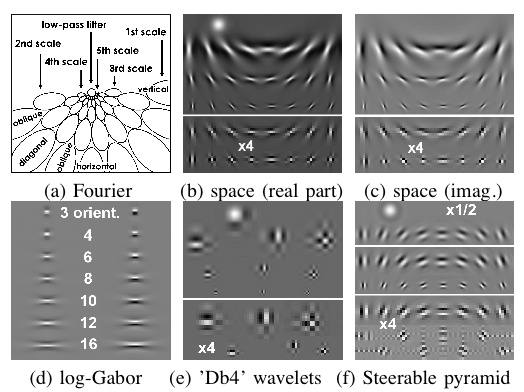
\includegraphics[width=.75\linewidth]{loggabor.png}%
\end{center}
\vfill%
[Fischer et al, 2007, International Journal of Computer Vision]%
\note{%%
	 in order to do that, we first used a linear transformation using a log-gabor representation
	 \begin{itemize}
		 \item[(definition)] this representation is a good and generic model of edges as defined by their shape, orientation and scale. It matches what is well described for the response of simple cells' response in area V1.  we show here on the top left that these filters tile evenly the Fourier space, but also that these correspond to a good model of edges at different orientation, scale and phase compared to other dictionaries like the Daubechies wavelet base Db4 in (e) and the steerable pyramid by Eero Simoncelli,
		  \item[(Fischer)] obviously, this dictionary is over-complete, but their correlation is easy to compute and allow for a relative translation-rotation-scale invariance. we proved that this was better adapted to the extraction of edges than gabors (Fischer, 07).
	\end{itemize}
	}%
}%
%
\subsection{Sparse coding}%
\frame[label=method3]{%
\frametitle{\insertsubsection}%
\begin{center}
	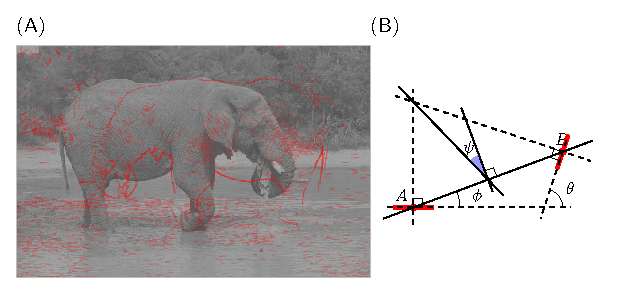
\includegraphics[width=\linewidth]{../ms/figure_model_ls.png}\\%
\end{center}
[LP (2003) IEEE TIP, LP (2015) BICV]%
\note{%%
	 \begin{itemize}
         \item[(MP)]  from this linear representation, we searched for the most sparse representation using a $\ell_0$ norm approach for which Matching Pursuit proved to be  a good approximation. I refer to this paper that appeared in IEEE TIP for more details
		 \item[(BICV)] and that i reviewed in a recent book chapter (Perrinet, 2015 bicv), including a model of complex cells' response (Fischer, 2007). It is generic and efficient. 
	\end{itemize}
	}%
}%

\subsection{Some examples of edge extraction}%
\frame[label=results1]{%
\frametitle{\insertsubsection}%
\begin{center}
\begin{changemargin}%
\begin{tabular}{cc}%
	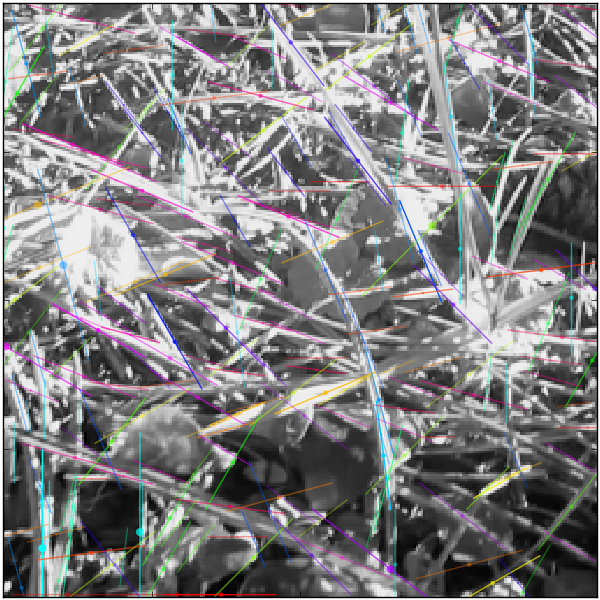
\includegraphics[width=.468\linewidth]{edgestats_vanilla_natural_frame570.png}&
	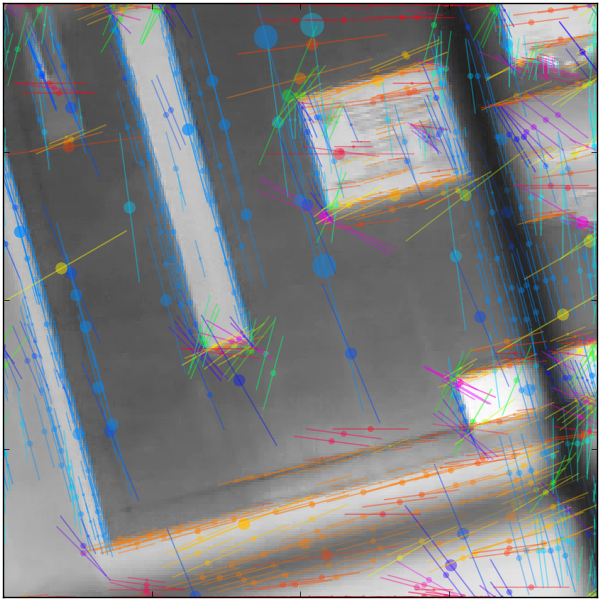
\includegraphics[width=.468\linewidth]{ms_laboratory_frame151.png}\\%
	Natural &%
	Laboratory %
\end{tabular}%
\end{changemargin}%
\end{center}
\note{%%
j
	\begin{itemize}
		 \item[(edges)] 	We show here the results of the edge extraction on a set of patches extracted from both database. Parameters for each edge are the scalar amplitude, position, phase, orientation and scale.  The hue gives the orientation, the length represents the size (scale) of the edge. This shows that edges are qualitatively well extracted. 
		\item[(efficient)] this method is rather general and proves to be efficiently grabbing most edges. in particular we can reconstruct the image from them and we achieved a performance measured by the RMSE of $\approx 5-10\% $
		\item[(qual)]  Both images classes appear qualitatively different and we tried to characterize how they differ. First-order statistics (distribution of positions, orientations, scale) showed a typical pattern but no differences between theses 2 classes... However, when computing...
	\end{itemize}
	}%
}%

\section{Results: natural vs. laboratory images}%
\begin{frame}%<beamer>
\frametitle{Outline: \Title}
\tableofcontents[currentsection]
\note{%
	let's now see the results of using such a method by 
	 \begin{itemize}
		 \item showing some examples of edge extraction
		 \item  computing second-order statistics
		 \item and trying to draw a quantitative measure of the difference between natural and laboratory images
		 \item database collection
	\end{itemize}
	}%
\end{frame}


%\subsection{Tracking behaviour}%
%\setbeamertemplate{background}
%{
%\begin{tikzpicture}%
%\draw [->,white,thick] (.9\textwidth,.9\textheight) -- (.95\textwidth,.95\textheight);
%\draw [->,white,thick] (0,.1\textheight) -- (0,.8\textheight) node[above, midway,sloped] {internal noise};
%\draw [->,red,thick] (.1\textwidth,0) -- (\textwidth,0) node [below,midway] {external noise};
%\end{tikzpicture}
%}
%

%\subsection{First-order statistics}%
%\frame[label=results2]{%
%\frametitle{\insertsubsection}%
%\includegraphics<1>[width=.5\linewidth]{../figures/edgestats_big_proba-theta_Yelmo.pdf}
%\includegraphics<1>[width=.5\linewidth]{../figures/edgestats_big_proba-theta_treeshrew.pdf}
%\begin{center}
%\end{center}
%\note{%%
%	We show here
%	}%
%}%

\subsection{Second-order statistics}%
\frame[label=results2]{%
\frametitle{\insertsubsection}%
\begin{center}%
\begin{changemargin}%
	\includegraphics<1|handout:0>[width=\linewidth]{../ms/figure_model_ls.png}%
	\includegraphics<2|handout:1>[width=.468\linewidth]{../ms/figure_chevrons.png}%
	\includegraphics<2|handout:1>[width=.468\linewidth]{schematics.pdf}%
	\includegraphics<3|handout:2>[width=.468\linewidth]{figure_chevrons_manmande.png}%
	\includegraphics<3|handout:2>[width=.468\linewidth]{schematics.pdf}%
\only<2-3|handout:1>{%
$$	 p( d, \psi, \theta, \sigma | \pi_0) \approx  p( d, \sigma  | \pi_0) p( \theta,\psi | \pi_0)  $$ 
}%
\end{changemargin}%
\end{center}%
\note<handout:1>{%
	... second-order stats, we will see a clear difference. The histogram was computed as a a 4-dimensional function of distance, azimuth $\psi$, difference of orientation $\theta$ and ratio of scale.
	\begin{itemize}
		 \item[(colin)]  let's first replicate the result from Geisler by showing that relative to a given edge (segment in the center), what is the Here I show for each distance and angle the most probable difference of angle, showing that collinear and parallel edges predominate. 
		\item[(lab)] when using the images from the laboratory environment, one finds a different pattern where the colinearity clearly dominates: this quantitatively shows the difference between the edges's second-order statistics... % Obviously, this should have a consequence on 
		 \item[(cocir)] a similar pattern is observed the cocircular plot. it reproduces the results from Geisler on natural images, but laboratory environment shows a strong bias to colinearity. 	
	\end{itemize}
	}%
\note<handout:2>{%
	Probability distribution function of "chevrons" in natural and laboratory images
	\begin{itemize}
		 \item[(angles)]  By computing measures of the independence of the different variables, we found that the probability density function of the second-order statistics of edges factorizes with on one side distance and scale and on the other side the 2 angles. The first component proved to be quite similar across both classes and the greater difference is seen for different angle configuration. As it can be reduced to 2 dimensions, we can plot the full probability as shown here by different contrast values assigned to all possible chevrons configurations, for all possible "azimuth" values $\psi$ on the horizontal axis and difference of orientation $\theta$ on the vertical axis. Such a plot most strikingly shows the difference between these 2 classes.
	\end{itemize}
	one issue now that we can show the 2nd order statistics is to know if it would be possible to quantify such difference...
	}%
}%

\subsection{Quantitative difference using classification}%
\frame[label=results3]{%
\frametitle{\insertsubsection}%
\centerline{%
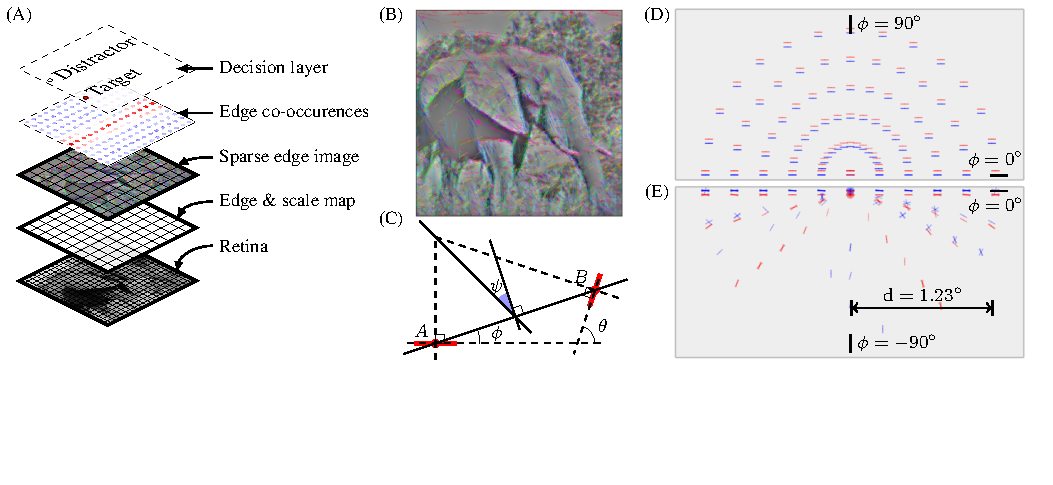
\includegraphics[width=\linewidth]{PerrinetBednar13-figure0.pdf}%
}%
\begin{table}[t]
\label{tab:results}
\begin{tabular}{llcccc}
 \multicolumn{1}{c}{\bf Database 1} &\multicolumn{1}{c}{\bf Database 2} &\multicolumn{1}{c}{\bf FO} &\multicolumn{1}{c}{\bf CM}&\multicolumn{1}{c}{\bf SO}
\\ \hline \\
% to update
Control & Man-made & 86\% & 92\% & 99\%\\
\end{tabular}
\end{table}
%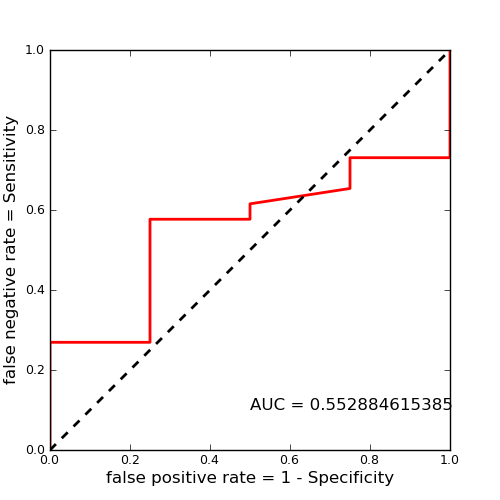
\includegraphics[width=.7\linewidth]{testing_smooth_KL_serre07_distractors_serre07_targets.png}%
\note{%%
%TODO : use SVN see p.33 of Dorr10phd
	\begin{itemize}
		 \item[(SVM)] ... we did that by using a simple classifier (a SVM classifier using the KL distance between the histogram of one image  to the average histogram to each class), so that one gets a simple, translation, orientation and scale invariant classifier which can efficiently differentiate between one natural image and a lab image. it comes as a big surprise as this is only based on some local characteristic, but it sufficient to get good classification. this gives also a quantitative method  to rate different methods and databases. The result as computed by f1-score is of 99.3\% accuracy.
		 \item[(animals)] as this ROC curve would be kind of boring to show (a right angle "perfect" wedge), we show one more surprising result: applying the same type of procedure to images of animals versus non-animals as used by the team of Simon Thorpe in Toulouse, one can get a pretty good classification of approximately 70\% accuracy. this comes as a surprise as we are only using a one-layer, feed-forward computation... still there is much to explore.
	\end{itemize}
	}%
}%
% -----------------------------------------------------------------------------------------------------------------------------------------------------
\subsection{Intermediate Summary}%
\frame[label=summary]{ %
\frametitle{\insertsubsection}%
\begin{changemargin}%
\begin{center}
\only<1|handout:0>{%
\begin{tabular}{cc}%
	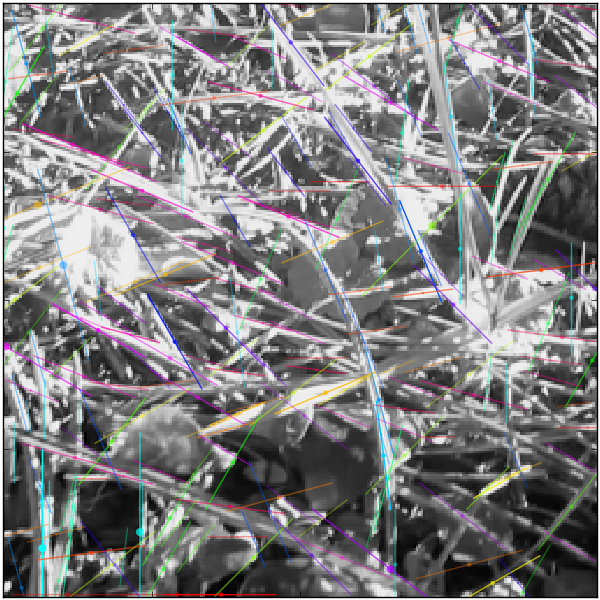
\includegraphics[width=.468\linewidth]{edgestats_vanilla_natural_frame570.png}&%
	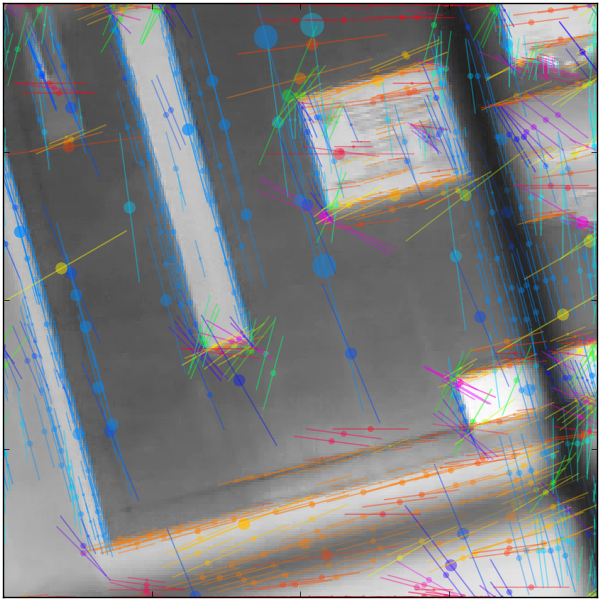
\includegraphics[width=.468\linewidth]{ms_laboratory_frame151.png}\\%
Natural &%
Laboratory %
\end{tabular}
}%
\only<2|handout:1>{%
$$	 p( d, \psi, \theta, \sigma | \pi_0) \approx  p( d, \sigma  | \pi_0) p( \theta,\psi | \pi_0)  $$ \\
\begin{tabular}{cc}%
	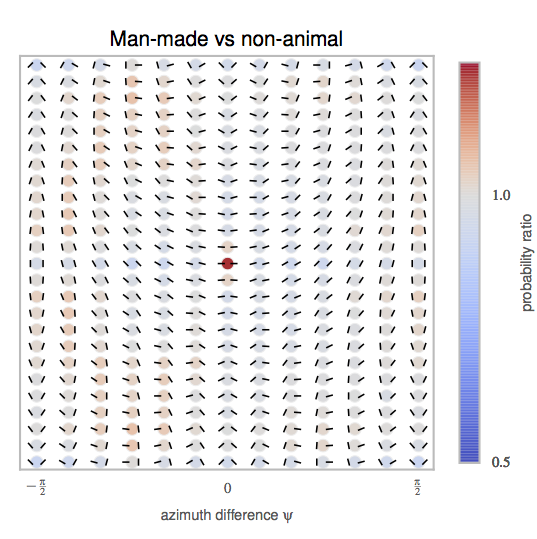
\includegraphics[width=.468\linewidth]{figure_chevrons_manmande.png}&%
	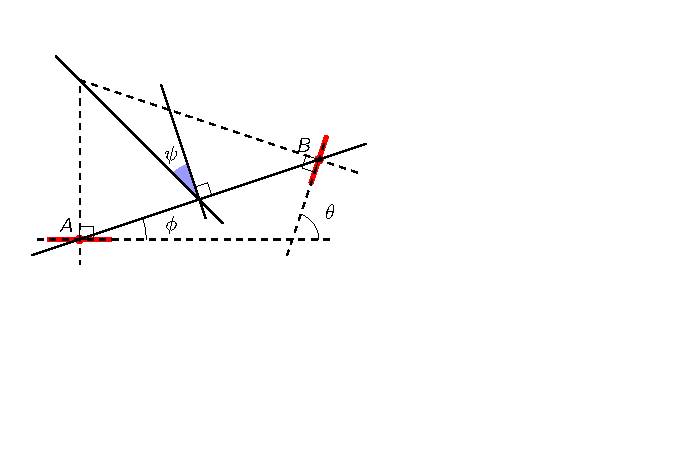
\includegraphics[width=.468\linewidth]{schematics.pdf}%
\end{tabular}
	}%
\end{center}
\end{changemargin}%
%
\note{%
%|  > 
%|  > I'd be interested in having more general discussion at the end about
%|  > what these results mean, and what should be done about them.  We have
%|  > to be careful not to assume that they represent plasticity, as we have
%|  > only circumstantial evidence of that, but we should mention plasticity
%|  > as a strong possibility.  I.e., we should say that the results are
%|  > highly suggestive of plasticity, given that the patterns of lateral
%|  > connectivity appear to be compatible with Hebbian learning of
%|  > cooccurence statistics of the animals' laboratory environment, but
%|  > that tests on wild-reared or differently reared animals (e.g. in cages
%|  > with wavy-line bars?) would need to be done to test that hypothesis.
%|  > And I think we should point out explicitly that meanwhile we should be
%|  > careful about interpreting the Bosking results as being representative
%|  > of neural implementations of natural scene statistics, as they appear
%|  > to be far more compatible with laboratory environment statistics.
To summarize, at this point of this talk  I hope I convinced you that 
	\begin{itemize}
		\item  \odot second-order statistics are efficiently computed by using a the algorithm from Geisler et al. (2001), with a more general edge extraction algorithm that uses sparse coding %to avoid multiple responses to a single edge. %using Matching Pursuit may be efficiently used to extract edges on natural images using an optimization of the matching step,
		\item \odot Collinearity and co-circularity results for natural images replicated qualitatively the results from Geisler et al. (2001), confirming that prior information about continuations appeared consistently in natural images. However, we find that the largely man-made environment in which these animals were reared has a significantly higher probability of collinear edge elements. % the second-order statistics of edges are very different in different environments and this may have consequences on the pattern of lateral interactions that is learned by the primary visual cortex due to plasticity and therefore on the results of Bosking and therefore on our understanding through models
		\item \odot We thus predict that if the lateral connection patterns are due to visual experience, the patterns in wild-raised tree shrews would be very different from those measured by Bosking et al. (1997), with shorter-range correlations and less emphasis on collinear continuations. This prediction can be tested in future experiments on matching groups of animals reared in different environments. $p(d,\sigma)$ should be hard-wired while $p(\theta, \psi)$ should be adaptive. cocircularity is weak but existent + anti-cocircularity is surprising= should be present as a connection structure. %these results may have some repercussions on edge extraction and we could use this prior knowledge to enhance the detection of edges (particles filtering)
		\item ... but, as we are here, may we try this on animals vs natural?...
	\end{itemize}
	} %
}
% -------------------------------------------------------------------------------------------------------------------
% -----------------------------------------------------------------------------------------------------------------------------------------------------
\section{Categorizing animals in images from natural scenes}%
\frame[label=serre07]{ %
\frametitle{\insertsection}%
\begin{changemargin}%
\begin{center}
\only<1|handout:0>{%
\begin{tabular}{cc}%
	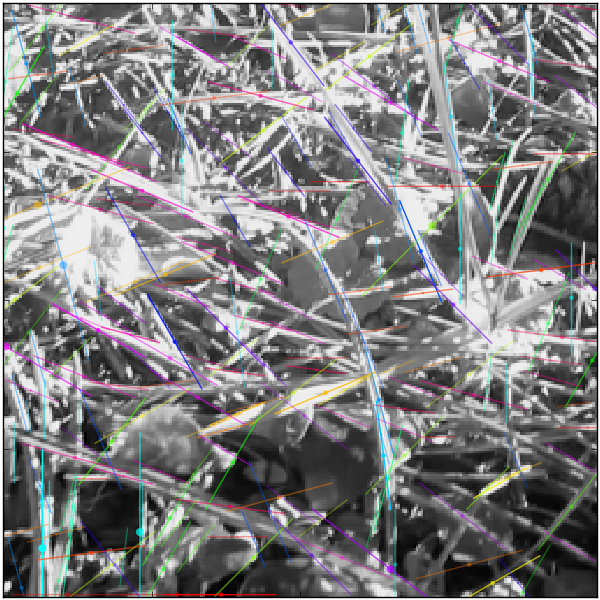
\includegraphics[width=.468\linewidth]{edgestats_vanilla_natural_frame570.png}&%
	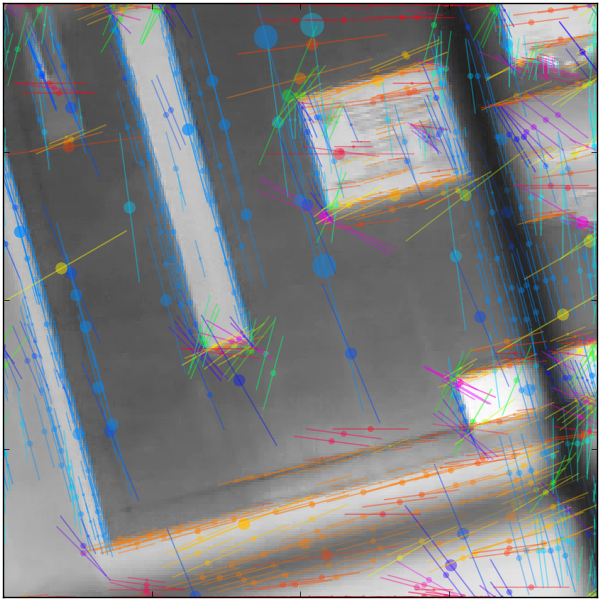
\includegraphics[width=.468\linewidth]{ms_laboratory_frame151.png}\\%
Natural &%
Laboratory %
\end{tabular}%
}%
\only<2|handout:0>{%
\begin{tabular}{cc}%
	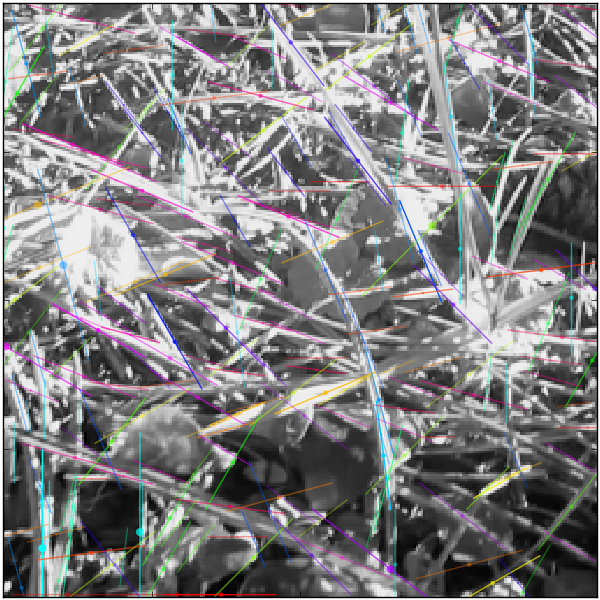
\includegraphics[width=.468\linewidth]{edgestats_vanilla_natural_frame570.png}&%
	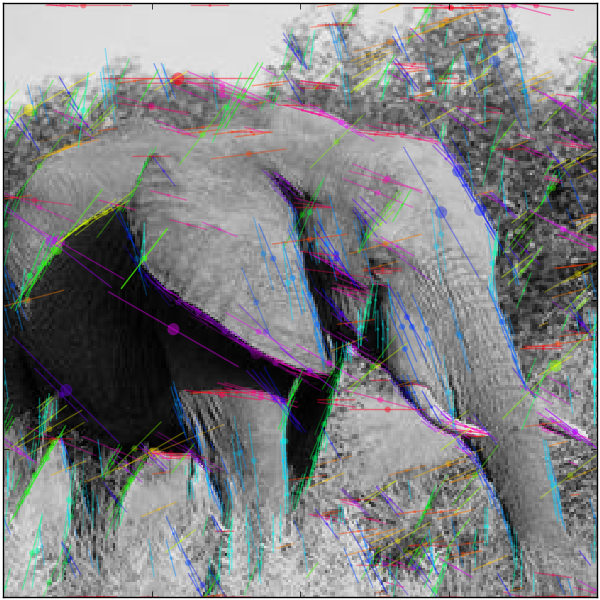
\includegraphics[width=.468\linewidth]{serre07_targets_B_N107001.png}\\%
Natural &%
Animal %
\end{tabular}%
}%
\only<3|handout:1>{%
	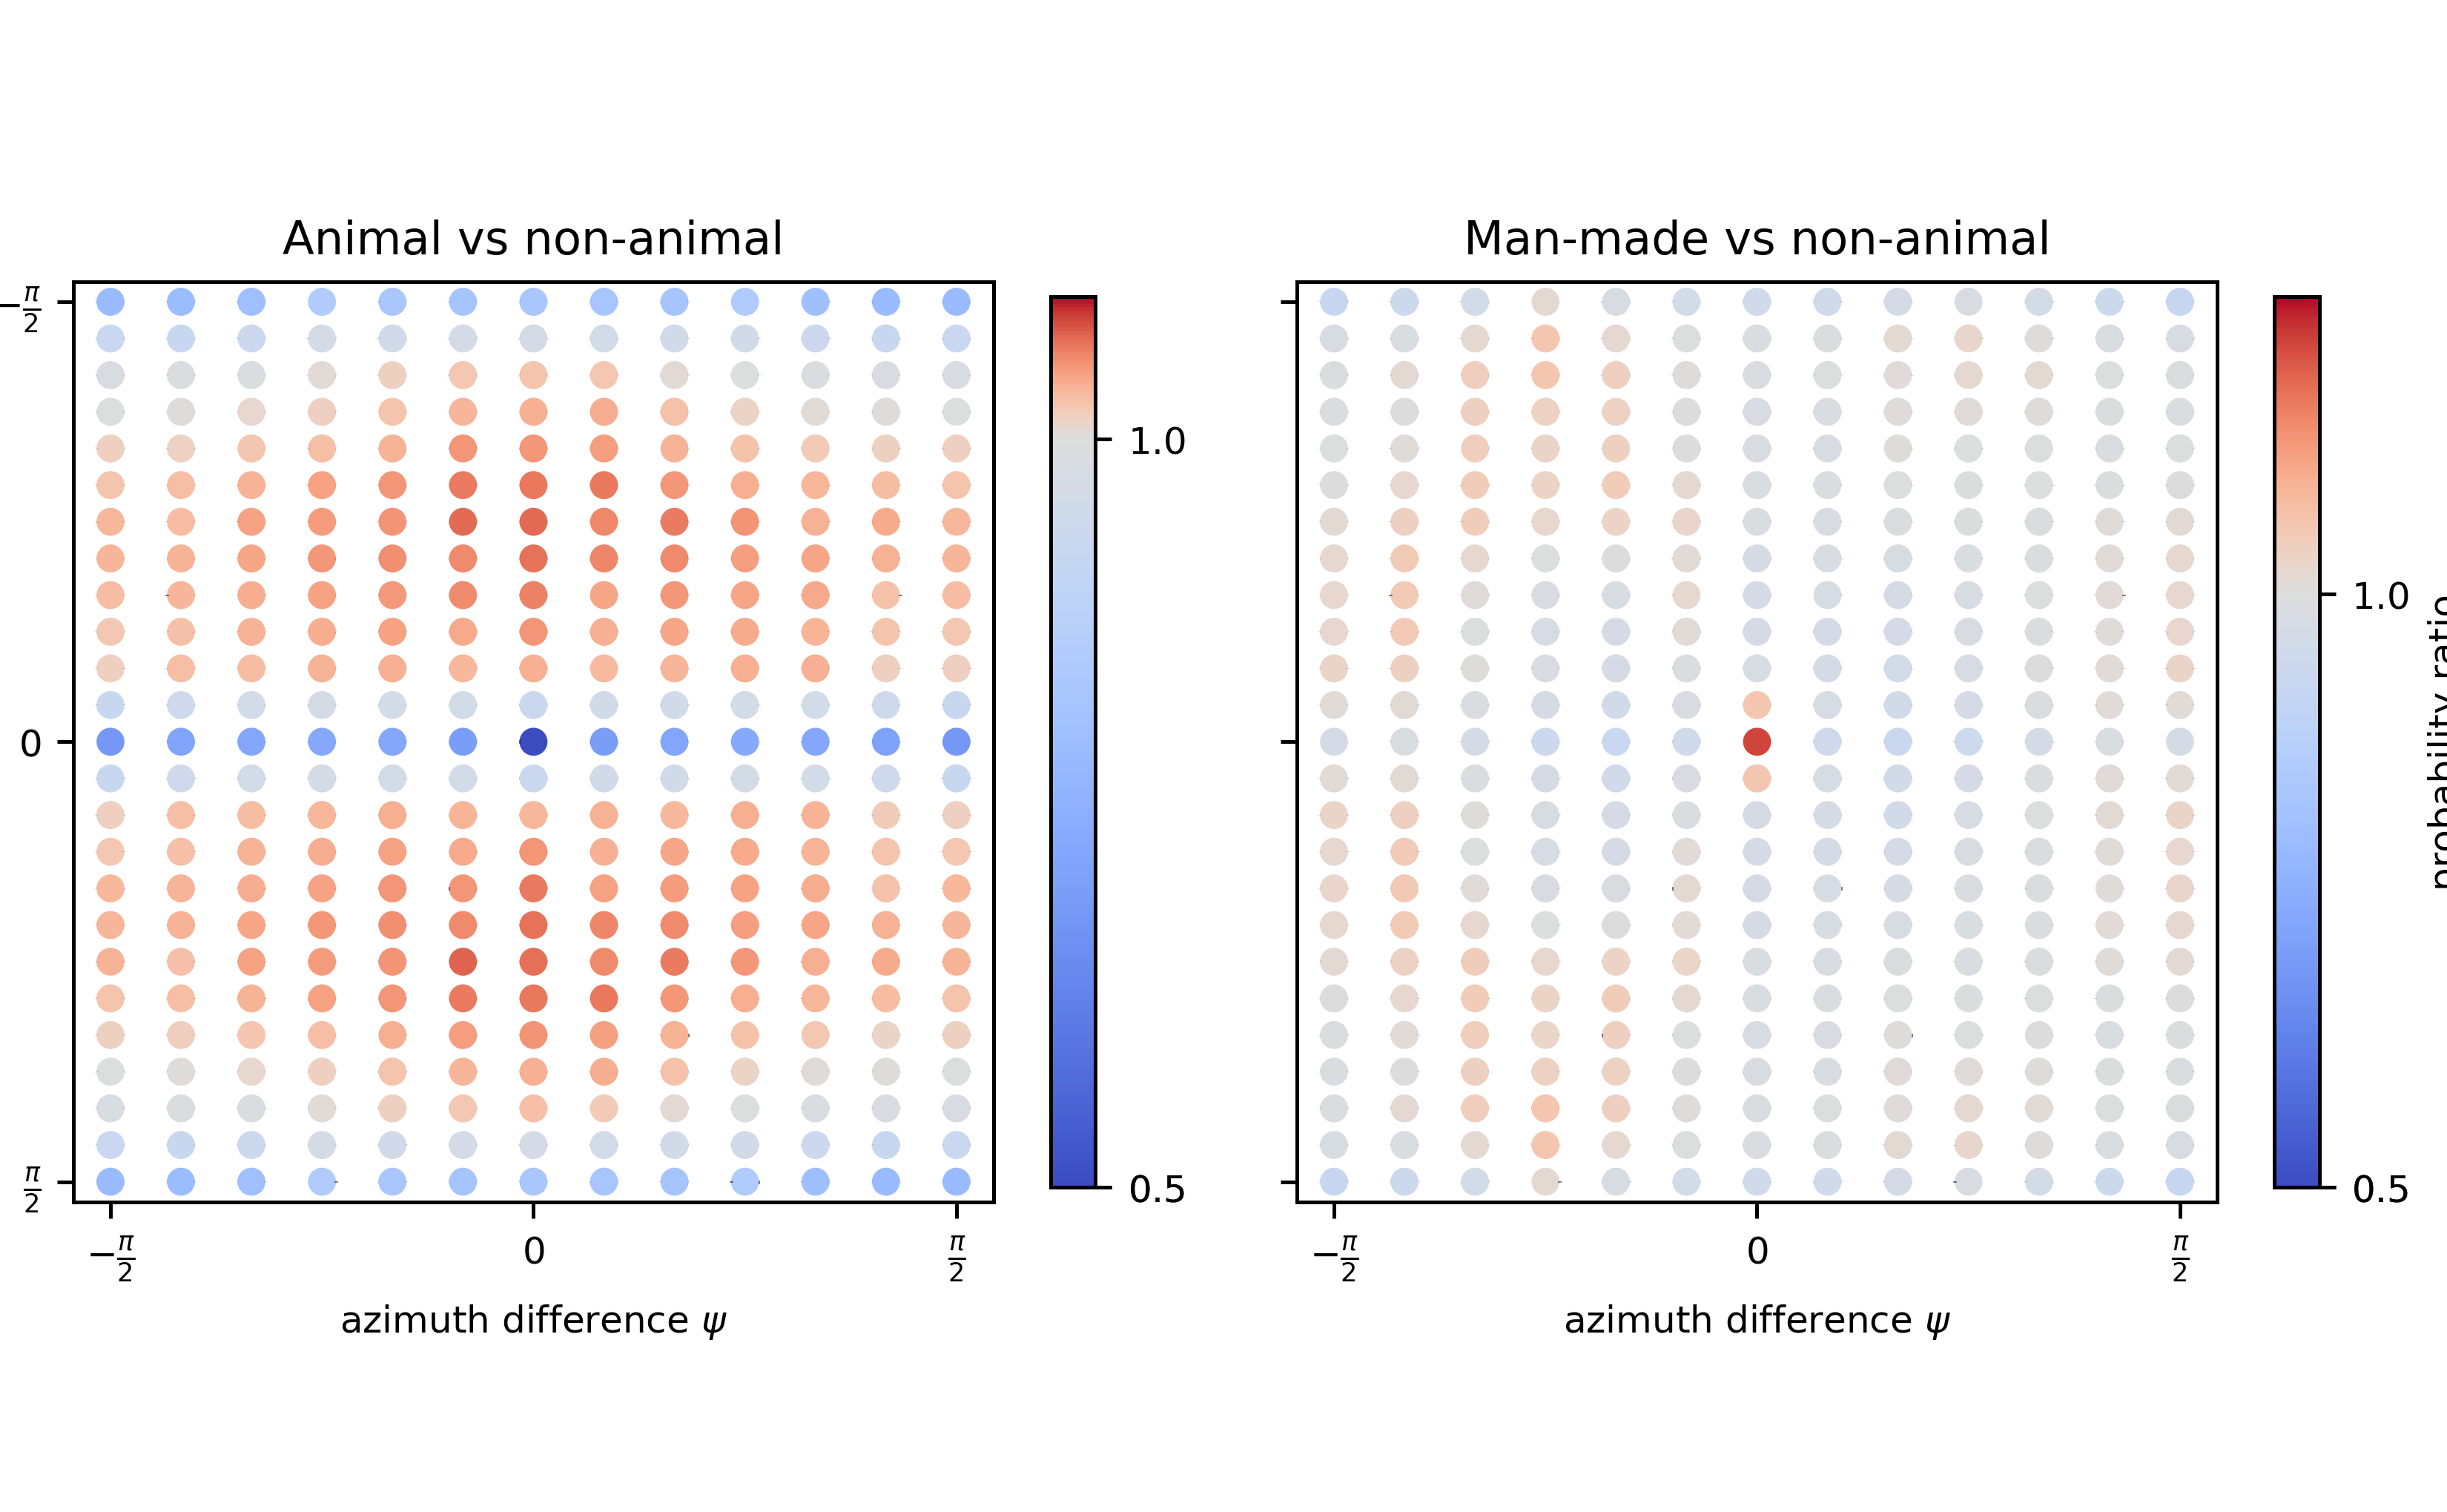
\includegraphics[width=\linewidth]{../ms/figure_chevrons2.png}%
	}%
\only<4|handout:2>{%
	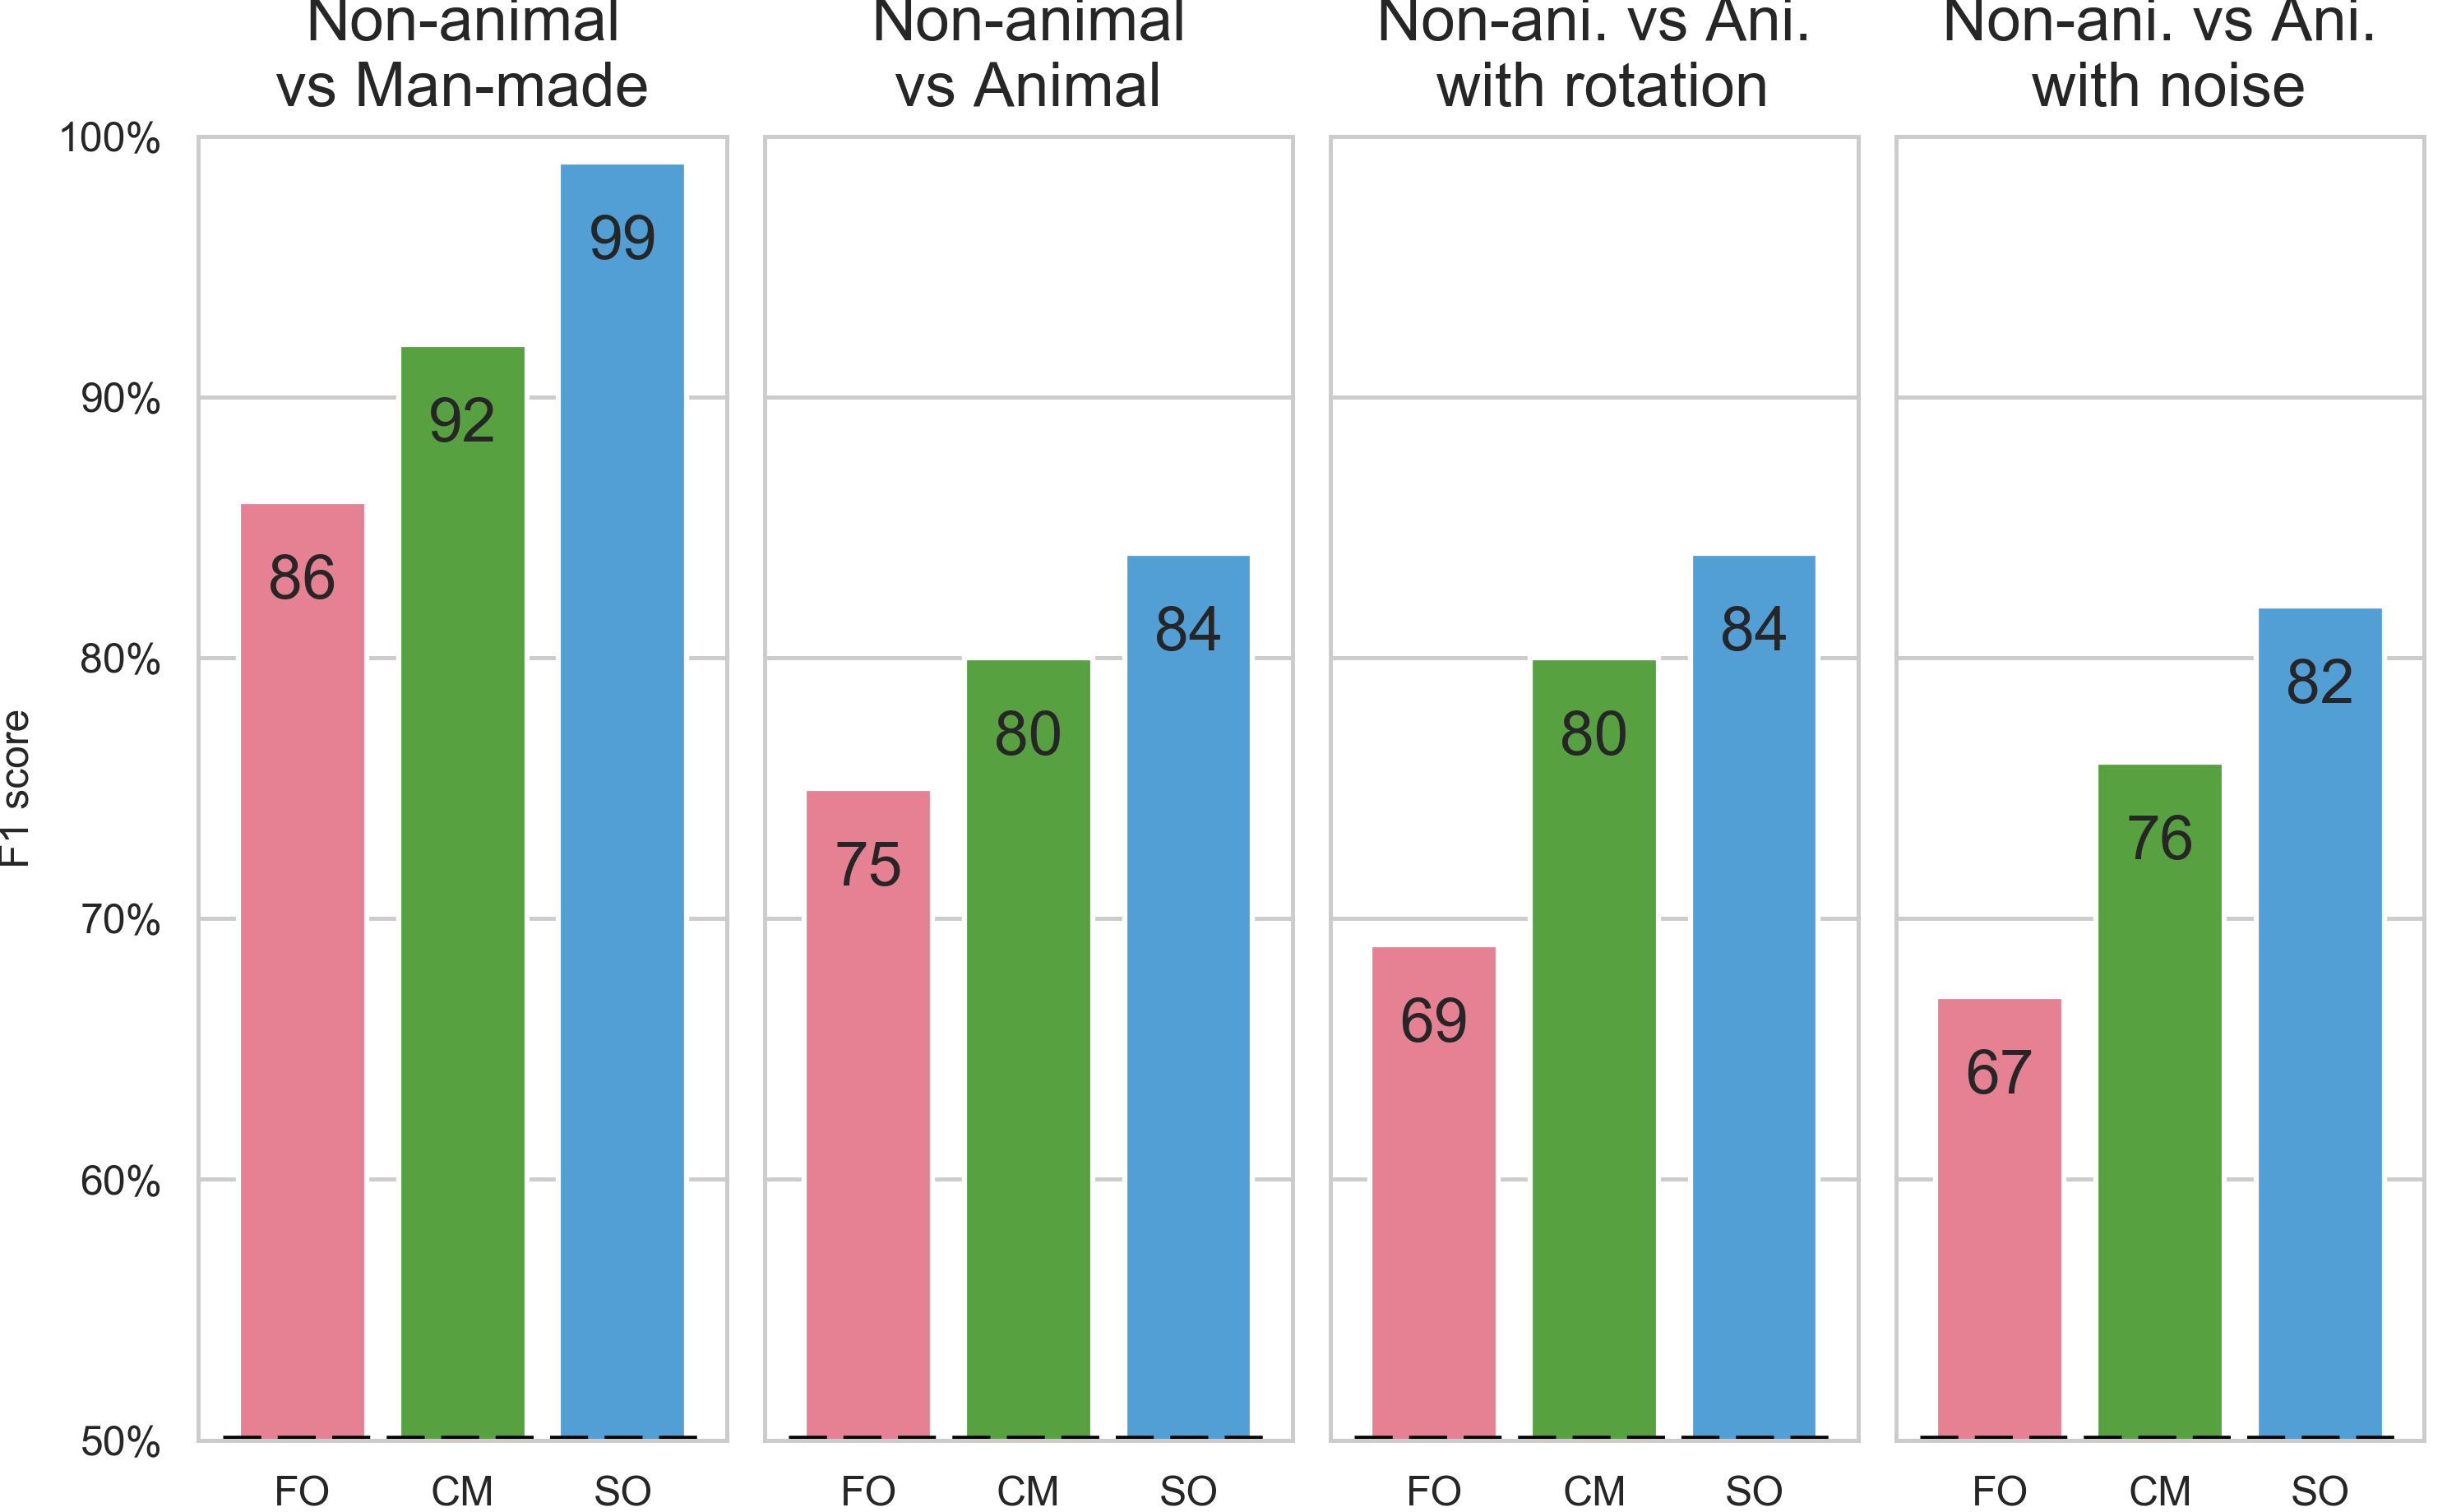
\includegraphics[width=.8\linewidth]{../ms/figure_results.png}%
}%
\only<5|handout:0>{%
	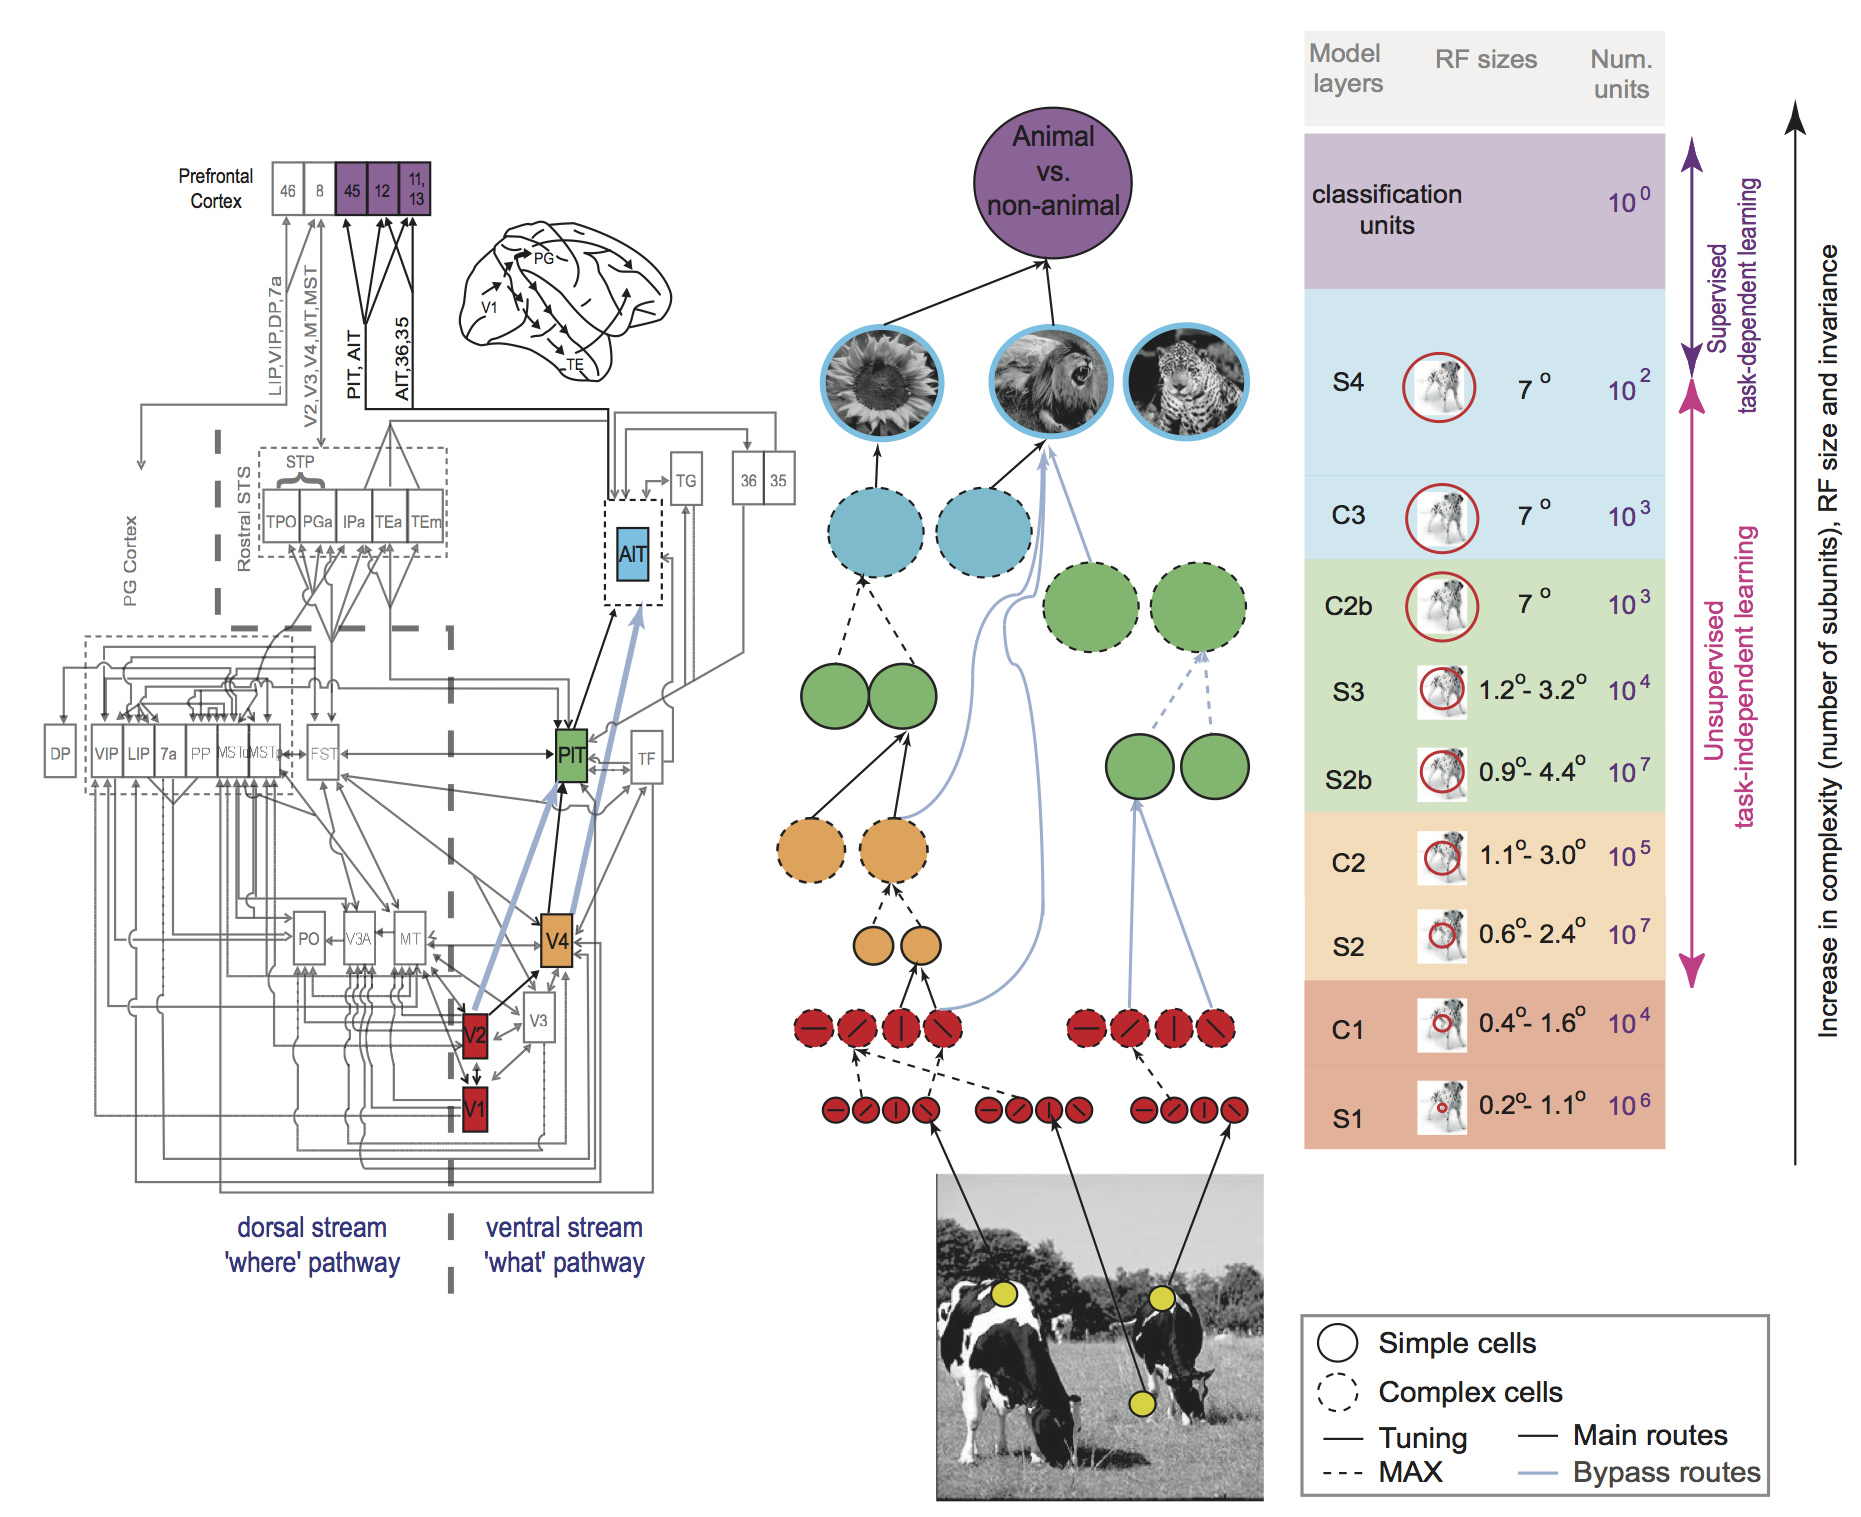
\includegraphics[width=.65\linewidth]{serre07fig1.png}%scheme_thorpe.jpg
	}%
\only<6|handout:3>{%
	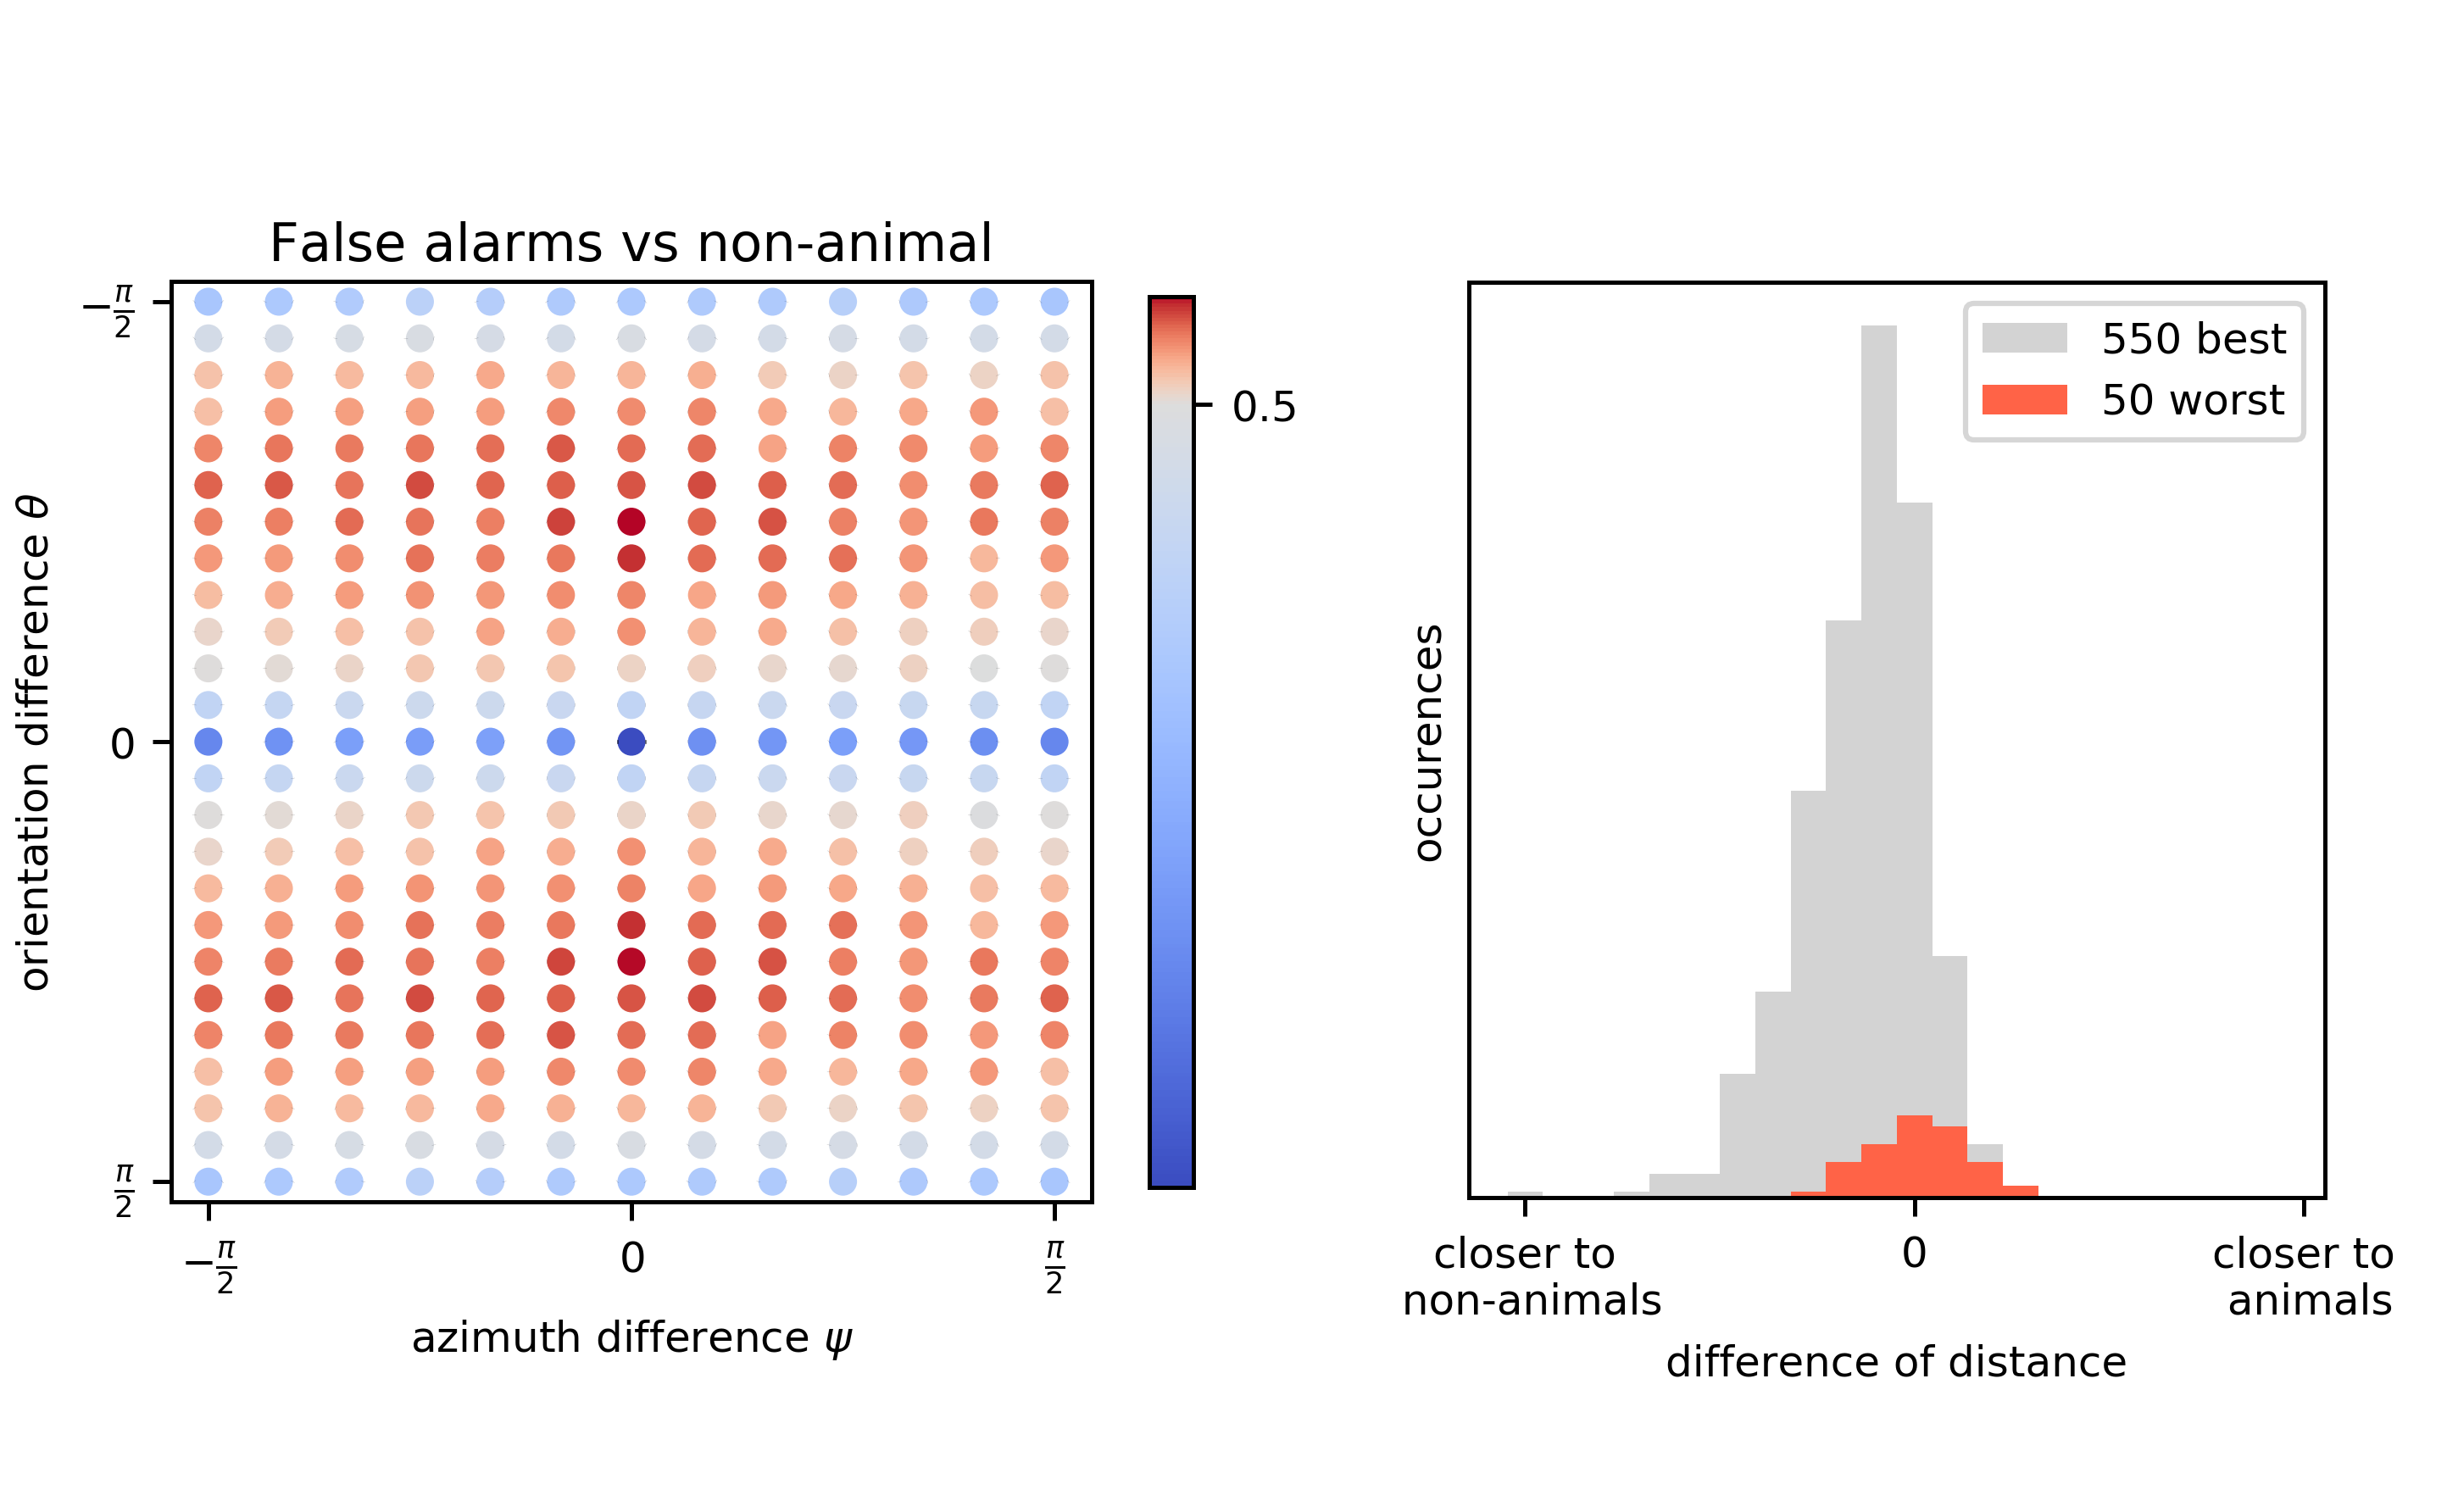
\includegraphics[width=.9\linewidth]{../ms/figure_FA_humans.png}%scheme_thorpe.jpg
	}%	
\only<7|handout:4>{%
\begin{tabular}{cc}%
	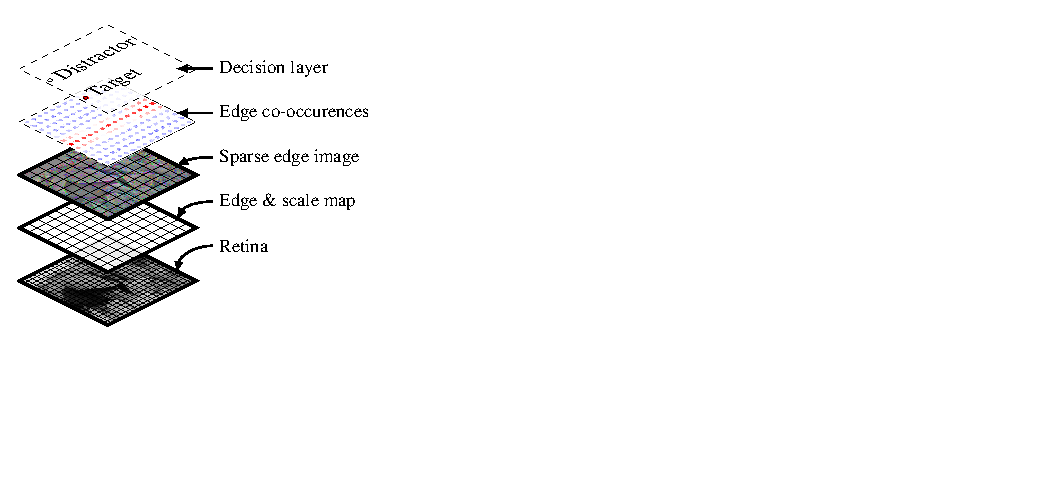
\includegraphics[width=.468\linewidth]{PerrinetBednar13-figure1A.pdf}&%
	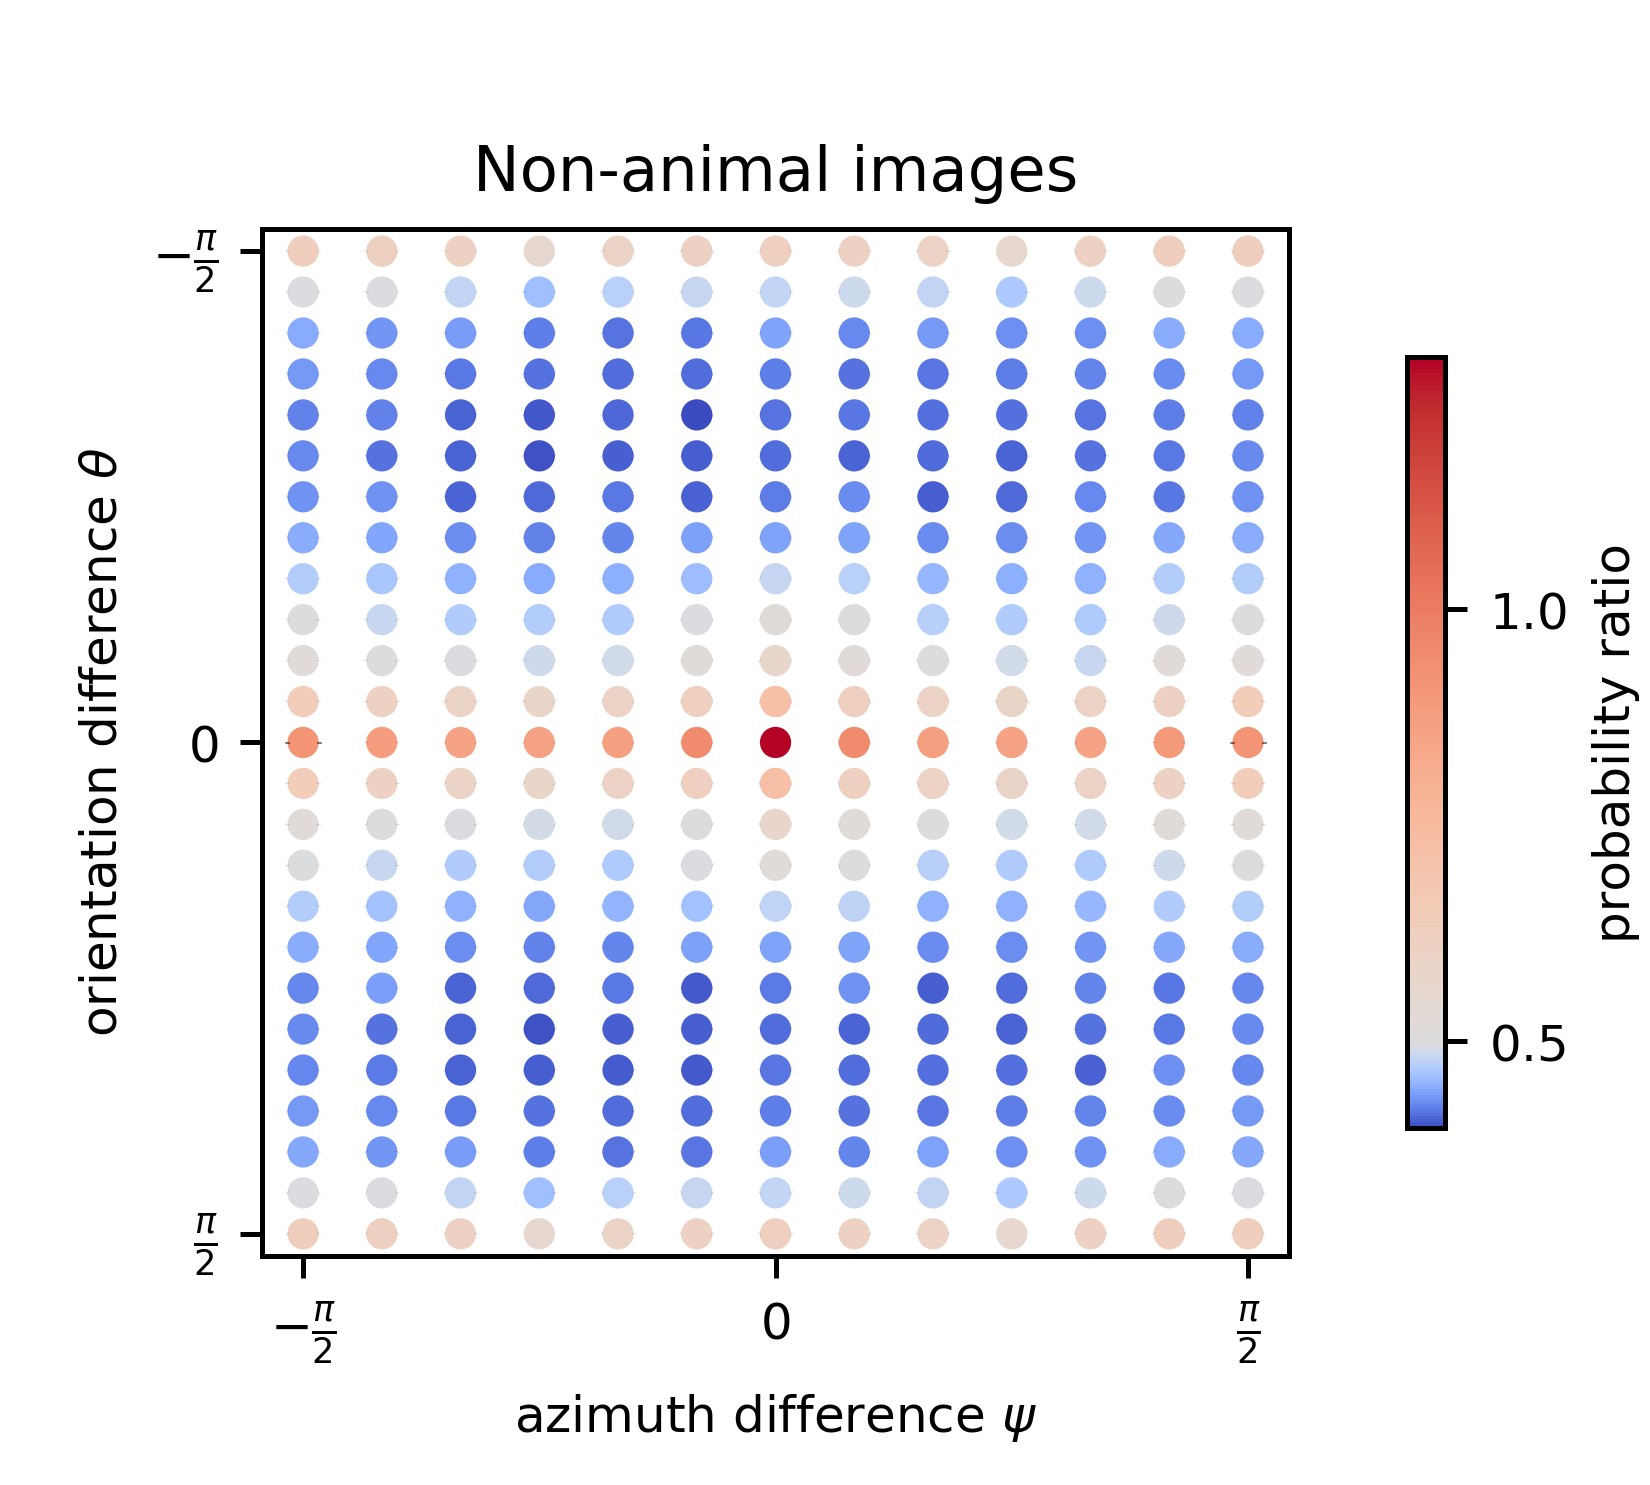
\includegraphics[width=.468\linewidth]{../ms/figure_chevrons.png}%
\end{tabular}%
%	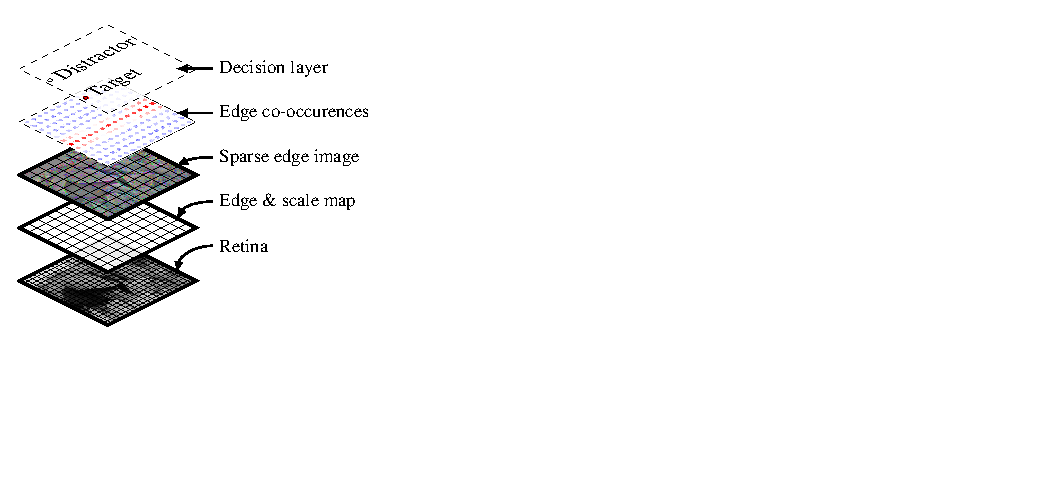
\includegraphics[width=.5\linewidth]{PerrinetBednar13-figure1A.pdf}%
	%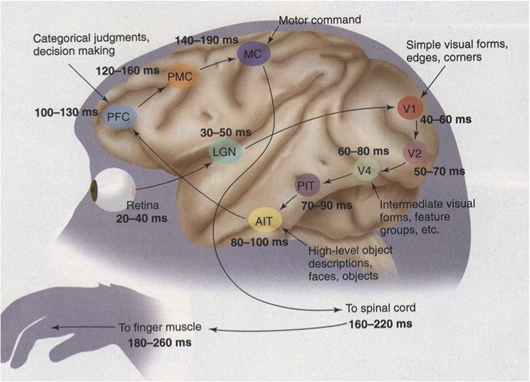
\includegraphics[width=.8\linewidth]{scheme_thorpe.jpg}%
	}%
\end{center}
\end{changemargin}%
%
\note<handout:1>{%

	\begin{itemize}
		\item \odot so if it works for calssiffying natural vs laboratory images, shouldn't it work for the task that Simon Thorpe as extensively studied, that is categorizing natural images \odot with or without an animal? This seems a bit crazy especially, knowing that most model (like the one from Serre 07) would rather consider that it is better done in 10 processing layers. But... let's just do it!
		\item \odot Let's show the Ratio of probability distribution function of chevron maps in artificial and animal images compared to the 'natural' set. As previously, we show the probability of chevron maps for two databases (artificial, animal), but here we compare this density to natural images by plotting the log-ratio of densities. These plots highlight the differences with natural images and shows the deviations in co-linearity for artificial images and in co-circularity for animal images (blue: less likely, red: more likely; the opacity is proportional to the absolute log-ratio). In this probabilistic framework, both high and low values carry information on the category of the image. 
	\end{itemize}
		}%
\note<handout:2>{%
	\begin{itemize}
		\item \odot Classification results for different sets of natural images (50\% is chance level) and different classification methods. Note that for SVM, we controlled for different feature choice: first-order statistics (SVM 1), full second-order statistics (SVM 2) or the chevron map only (SVM C). Surprisingly, the results are very similar to the results of Serre 07, and w do not lose much performance by choosing the simple chevron map. First, this has direct application in machine learning as this translation- and rotation-independent classifier performs as well as more complicated networks (that is they have more parameters) - and could be imported to architectures such as spikenet
		\item \odot but what can we conclude from that? It shows that compared to the view of the visual system as a single-track, feed-forward architecture (as shown in the is figure showing the architecture of Serre, 07), visual information can follow different, parallel, certainly redundant routes that will allow to optimize the efficiency of the system. These systems may work in synergy and challenges the dichotomy between analytical vs global representations: it rather seems that with the brain, much is possible. This is certainly useful to learn more about the adaptivity and generality of neural computations.
	\end{itemize}
	} 
\note<handout:3>{%
	\begin{itemize}
		\item \odot To see whether the patterns of errors made by humans are consistent with our model, we studied the second-order statistics of the 50 non-animal images that human subjects in Serre et al. (2007) most commonly falsely reported as having an animal. We call this set of images the false-alarm image dataset. (Left) This chevron map plot shows the ratio between the second-order statistics of the false-alarm images and the full non-animal natural image dataset, computed as in Figure 3 (left). Just as for the images that actually do contain animals (Figure~\ref{fig:chevrons2}, left), the images falsely reported as having animals have more co-circular and converging (red chevrons) and fewer collinear and orthogonal configurations (blue chevrons). (Right) To quantify this similarity, we computed the Kullback-Leibler distance between the histogram of each of these images from the false-alarm image dataset, and the average histogram of each class. The difference between these two distances gives a quantitative measure of how close each image is to the average histograms for each class. Consistent with the idea that humans are using edge co-occurences to do rapid image categorization, the 50 non-animal images that were worst classified are biased toward the animal histogram ($d' = 1.04$), while the 550 best classified non-animal images are closer to the non-animal histogram.
	\end{itemize}
	} 
\note<handout:4>{%
	\begin{itemize}
		\item \odot To conclude... These results call into question previous claims that a hierarchical
analysis of the visual scene is necessary 
for classification into high-level categories (Serre, 07)
We speculate that the observed differences in second-order statistics for images
with animals have an underlying basis in the physical constraints 
governing the shapes of animals. 
Specifically, animals typically have compact shapes, constrained by
their capacity to move, unlike plants rooted
in one location that must stretch rather than move towards resources.
 Thus we expect that the second-order statistics will be useful
as a rough but general and fast method for distinguishing a wide range
of scene and object categories.  Similar observations apply to other
sensory systems, where we would expect co-occurence between primary
sensory elements (such as stimulation of a patch of skin, presence of
a specific auditory frequency, or activation of a taste or smell
receptor) to differ between ecologically important classes of stimuli.
	\end{itemize}	
	Thank you for your attention.
	} 

}
%
%\usebackgroundtemplate{%
%\includegraphics[width=.7\paperwidth]{empty.png}%
%\includegraphics[width=.3\paperwidth]{qrcode.png}%
%}%
%
%\subsection*{References}%
\frame[label=biblio]{%\frametitle{References}%\insertsubsection}%

%\begin{tikzpicture}[remember picture,overlay]  
%  \node [xshift=-.2\paperwidth,yshift=.3\paperwidth] at (current page.south east)
%    { \includegraphics[width=.3\paperwidth]{qrcode.png}  \end{center} };
%\end{tikzpicture}

{\tiny
\begin{thebibliography}{5}
%\providecommand{\url}[1]{\texttt{#1}}
%\expandafter\ifx\csname urlstyle\endcsname\relax
%  \providecommand{\doi}[1]{doi: #1}\else
%  \providecommand{\doi}{doi: \begingroup \urlstyle{rm}\Url}\fi

\bibitem[Geisler et~al.(2001)]{Geisler01}
W.~Geisler, J.~Perry, B.~Super, D.~Gallogly
\newblock {E}dge co-occurence in natural images predicts contour grouping performance.
\newblock \emph{Vision Research}, 41:\penalty0 711--24, 2001.

\bibitem[Field et~al.(1993)]{Field1993}
D.~Field and A.~Hayes and R.~Hess
\newblock Contour integration by the human visual system: evidence for a local "association field".
\newblock \emph{Vision Research}, 33\penalty0 (2):\penalty0 173--93, 1993.

\bibitem[Choe et~al.(2004)]{Choe2004}
Y. Choe and R. Miikkulainen
\newblock Contour integration and segmentation with self-organized lateral connections.
\newblock \emph{Biological Cybernetics}, 90\penalty0 (2):\penalty0 75--88, 2004.

\bibitem[Bosking et~al.(1997)]{Bosking97}
W.~Bosking, Y.~Zhang, B.~Schofield, and D.~Fitzpatrick
\newblock  Orientation selectivity and the arrangement of horizontal connections in tree shrew striate cortex
\newblock \emph{The Journal of Neuroscience}, 17\penalty0 (6):\penalty0 2112-27, March 15, 1997.
%
\bibitem[Callaway, E. M. and Katz, L. C.]{Callaway90}
E.~Callaway and L.~Katz
\newblock Emergence and refinement of clustered horizontal connections in cat striate cortex.
\newblock \emph{The Journal of Neuroscience}, 10\penalty0 (4):\penalty0 1134--53, 1990.

\bibitem[Fischer et~al.(2007)Fischer, \v{S}roubek, Perrinet, Redondo, and  Crist{\'{o}}bal]{Fischer07a}
S.~Fischer, F.~\v{S}roubek, L.~U. Perrinet, R.~Redondo, and G.~Crist{\'{o}}bal.
\newblock {Self-Invertible 2D Log-Gabor Wavelets}.
\newblock \emph{International Journal of Computer Vision}, 75\penalty0 (2):\penalty0 231--246, 2007.
%\newblock \doi{http://dx.doi.org/10.1007/s11263-006-0026-8}.
%\newblock URL  \url{http://dx.doi.org/http://dx.doi.org/10.1007/s11263-006-0026-8}.
%\newblock URL  \url{\Website/Publications/Fischer07}.

\bibitem[Perrinet(2010)]{Perrinet10shl}
L.~U. Perrinet.
\newblock {Role of homeostasis in learning sparse representations}.
\newblock \emph{Neural Computation}, 22\penalty0 (7):\penalty0 1812--36, July 2010.
%\newblock \doi{10.1162/neco.2010.05-08-795}.
%\newblock URL  \url{\Website/Publications/Perrinet10shl}.

\bibitem[Perrinet(2015)]{Perrinet13cerco}
L.~U. Perrinet, and J.~Bednar
\newblock {\SubTitle}.
\newblock \emph{Scientific Reports}, 2015.
\newblock URL  \url{\Website}%

\bibitem[Seri{\`e}s et~al.(2002)Seri{\`e}s, Georges, Lorenceau, and  Fr{\'e}gnac]{Series02}
P.~Seri{\`e}s, S.~Georges, J.~Lorenceau, and Y.~Fr{\'e}gnac.
\newblock {O}rientation dependent modulation of apparent speed: a model based on the dynamics of feed-forward and horizontal connectivity in {V}1 cortex.
\newblock \emph{Vision {R}esearch}, 42\penalty0 (25):\penalty0 2781--97, Nov 2002.


\end{thebibliography}}
}
%------------------------------------------------------------------%
\appendix
\section{\appendixname}
%
\frame[label=peggy]{%
\frametitle{Neuromorphic implementation}%
\begin{columns}%
\begin{column}{.5\textwidth}%
	\begin{center}%
		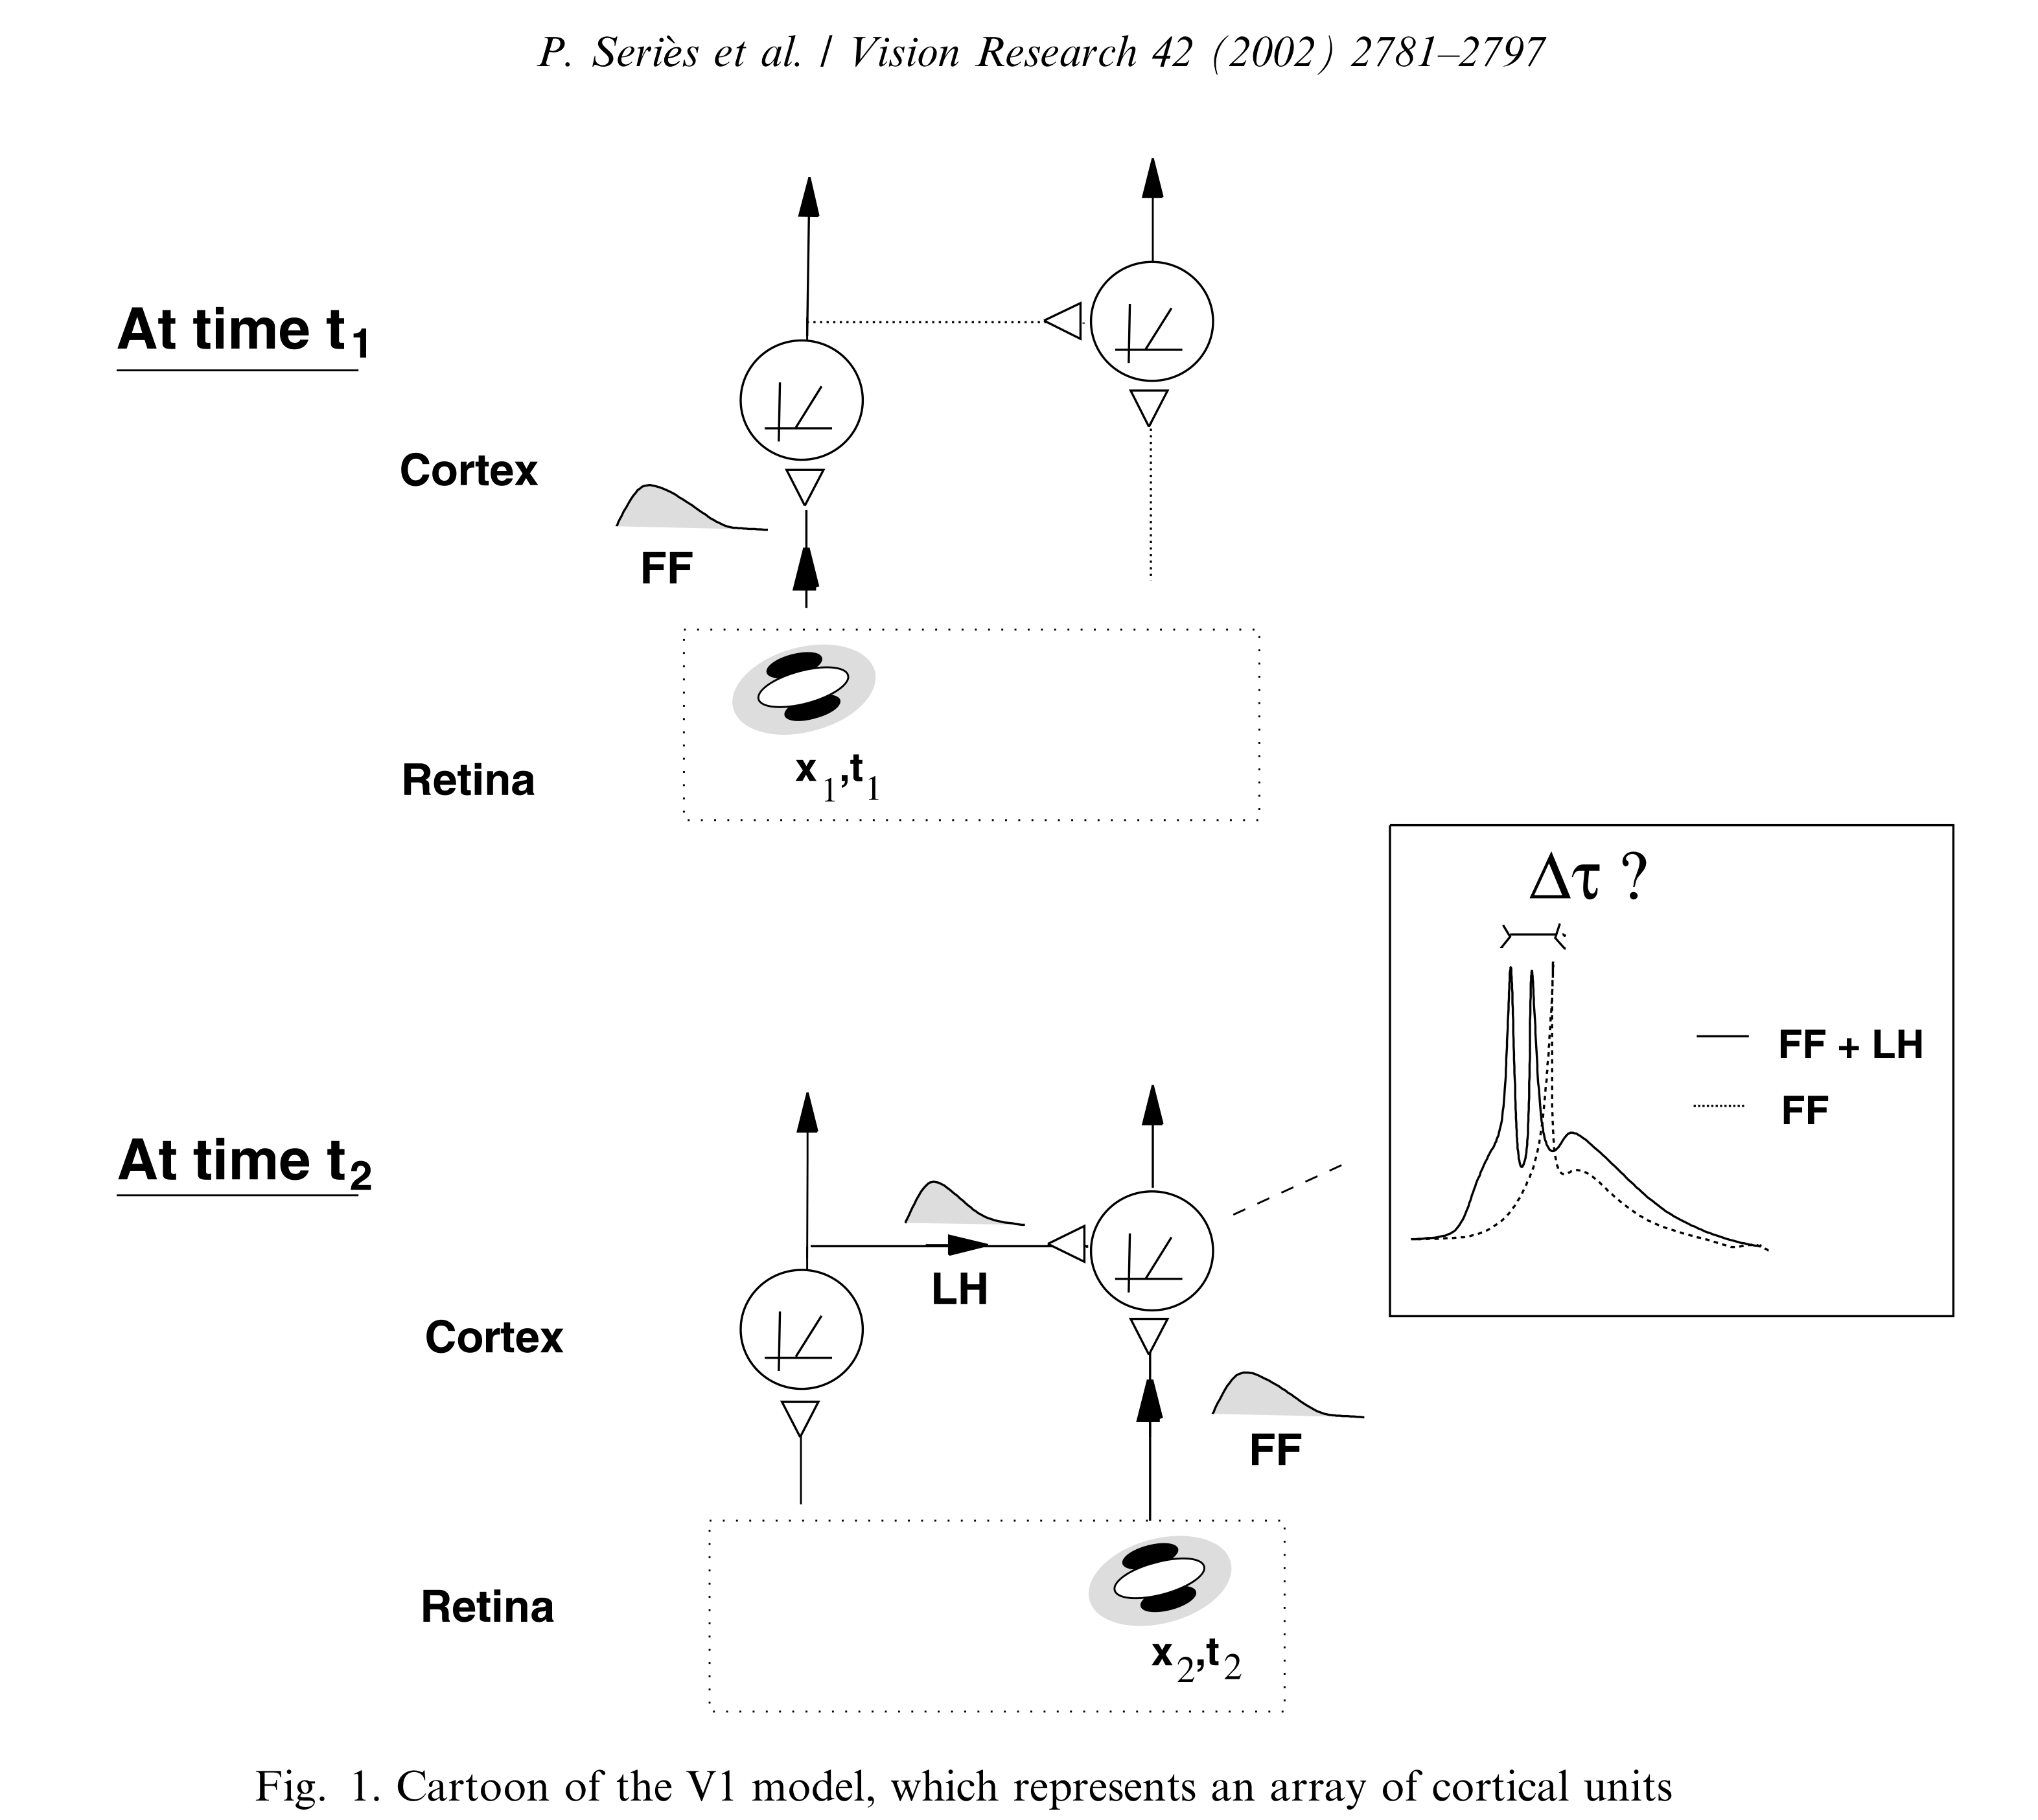
\includegraphics[width=.95\columnwidth]{figure_series.png}%\\%
	\end{center}%
\end{column}%
\begin{column}{.5\textwidth}%
	\begin{center}%
		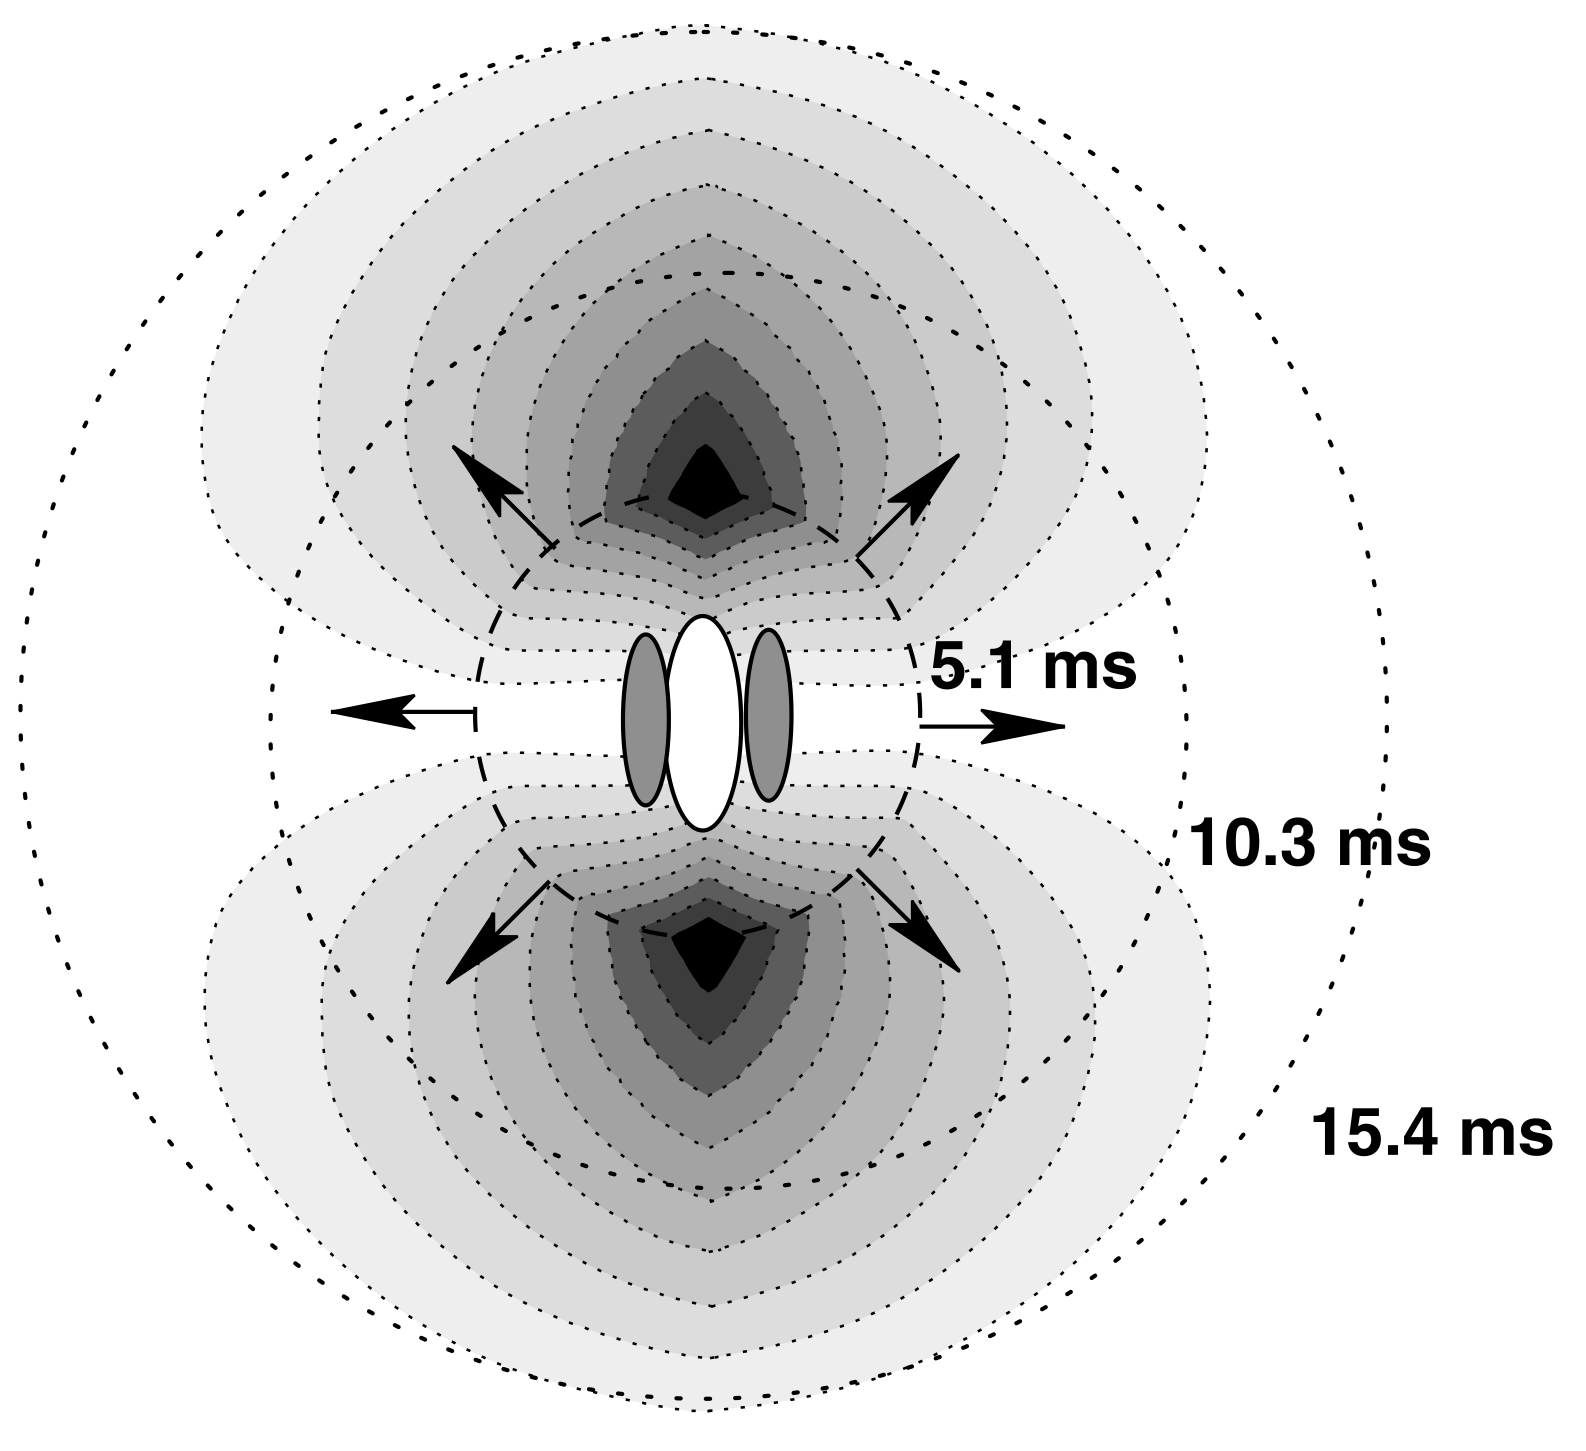
\includegraphics[width=.6\columnwidth]{figure_series_11.png}%
	\end{center}%
	[Series et al., 2002]
\end{column}%
\end{columns}%
}%
%
\frame[label=mp]{ %
\frametitle{Matching Pursuit}%
\begin{changemargin}%
\begin{center}
\only<+|handout:+>{%
	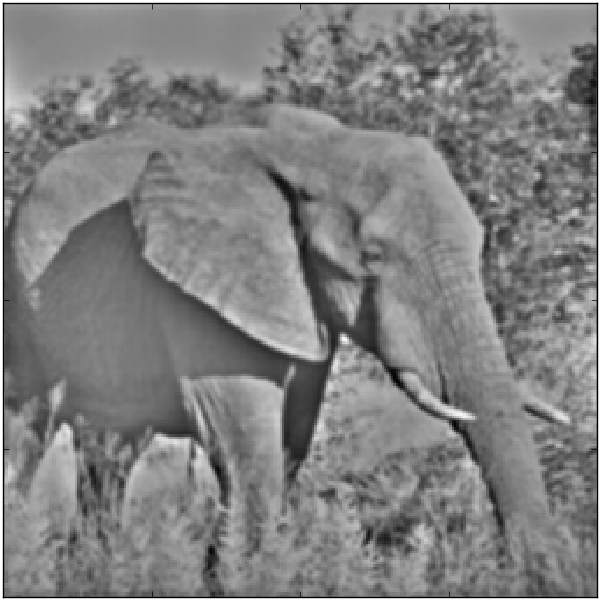
\includegraphics[width=.998\linewidth]{MP_0.png}%
}%
\only<+|handout:+>{%
	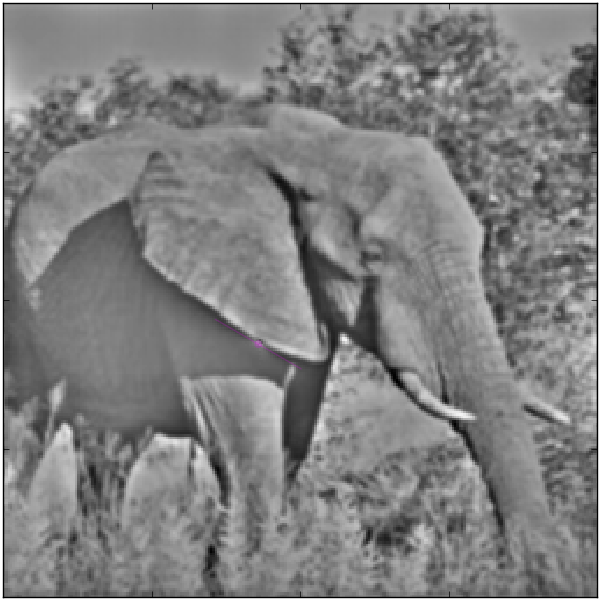
\includegraphics[width=.998\linewidth]{MP_1.png}%
}%
\only<+|handout:+>{%
	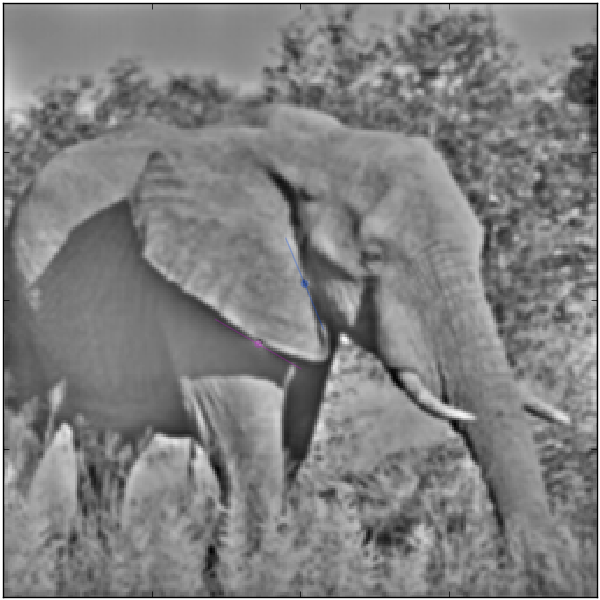
\includegraphics[width=.998\linewidth]{MP_2.png}%
}%
\only<+|handout:+>{%
	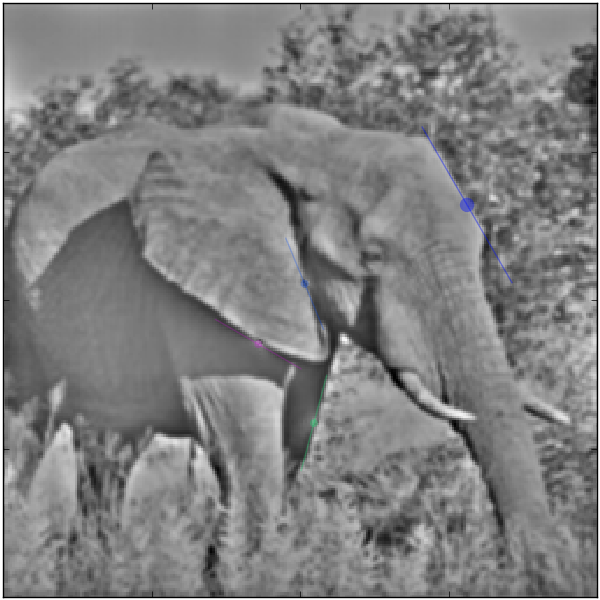
\includegraphics[width=.998\linewidth]{MP_4.png}%
}%
\only<+|handout:+>{%
	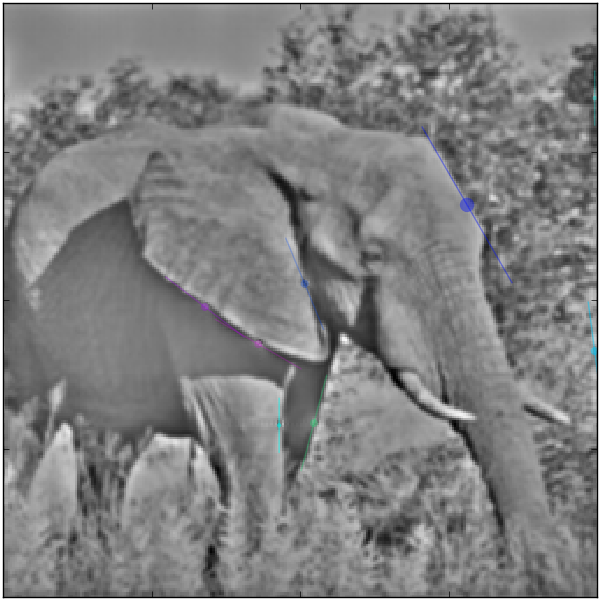
\includegraphics[width=.998\linewidth]{MP_8.png}%
}%
\only<+|handout:+>{%
	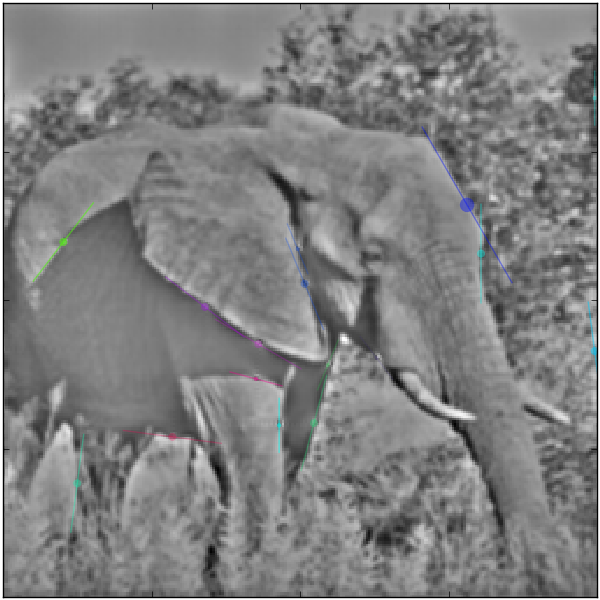
\includegraphics[width=.998\linewidth]{MP_16.png}%
}%
\only<+|handout:+>{%
	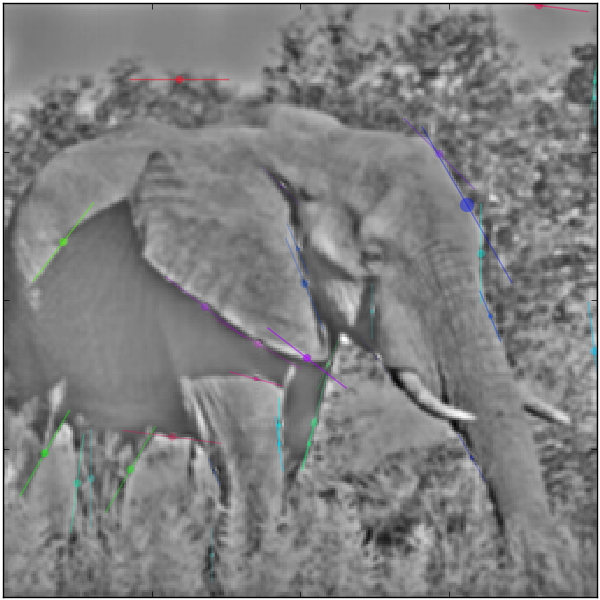
\includegraphics[width=.998\linewidth]{MP_32.png}%
}%
\only<+|handout:+>{%
	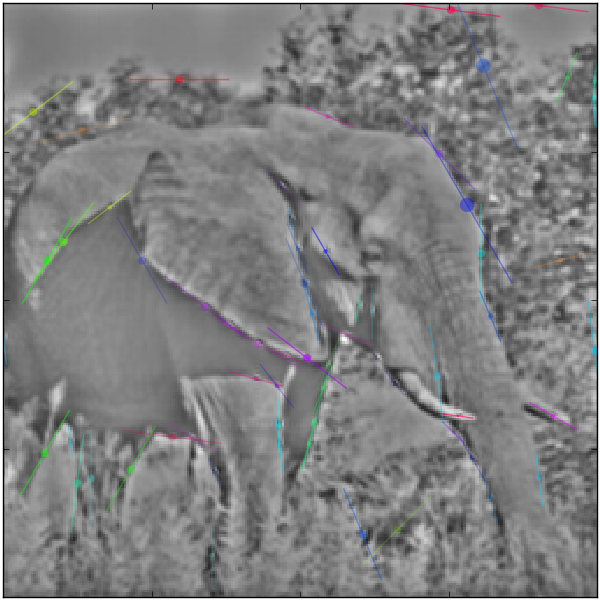
\includegraphics[width=.998\linewidth]{MP_64.png}%
}%
\only<+|handout:+>{%
	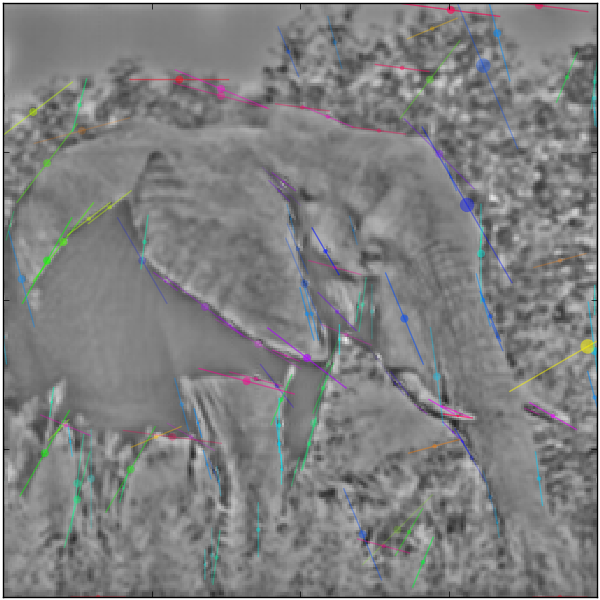
\includegraphics[width=.998\linewidth]{MP_128.png}%
}%
\only<+|handout:+>{%
	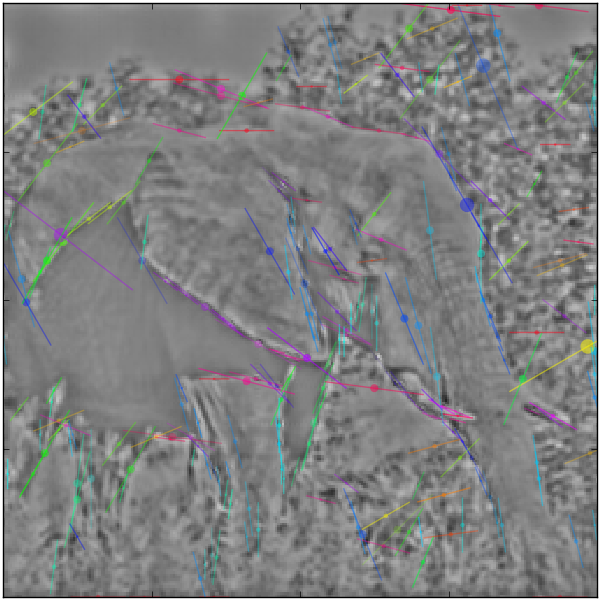
\includegraphics[width=.998\linewidth]{MP_256.png}%
}%
\only<+|handout:+>{%
	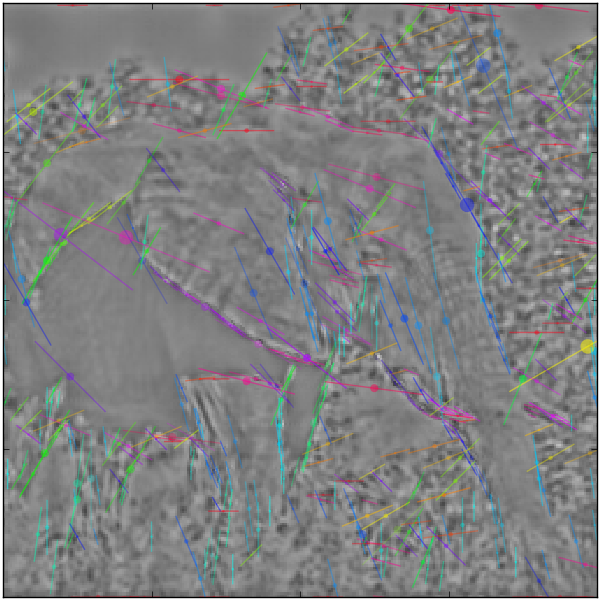
\includegraphics[width=.998\linewidth]{MP_512.png}%
}%
\only<+|handout:+>{%
	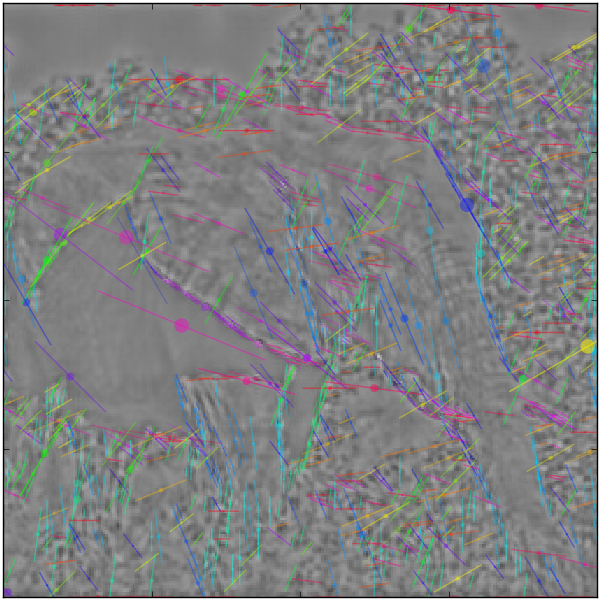
\includegraphics[width=.998\linewidth]{MP_1024.png}%
}%
\only<+|handout:+>{%
	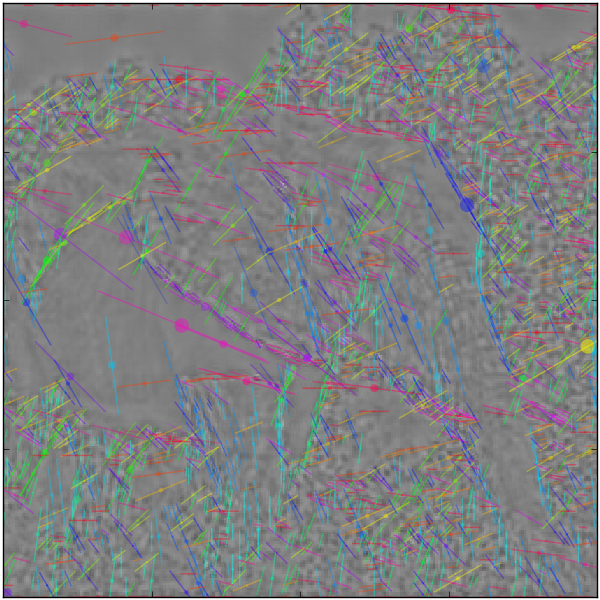
\includegraphics[width=.998\linewidth]{MP_2048.png}%
}%
\begin{tabular}{cc}%
Residual &%
Edges %
\end{tabular}%
\end{center}
\end{changemargin}%
%
%\note{%
%This is how Matching Pursuit works:
%	\begin{itemize}
%		\item on the left, ...	
%		\item at the first step...
%	\end{itemize}
%	} 
}%

%-------------------------------------------------------------------------------------------%
\end{document}%
